\section{Growth regimes: analytical results and numerical transitions}
\label{sec:axm-growth-regimes}

This section organizes the model's implications around four economically
distinct cases. Each case first states the analytical characterization and then,
when a validated computation is available under the present specification,
presents the corresponding numerical transition. The six cells in Table
\ref{tab:axm-regime-map} keep the roles of the two elasticities separate without
requiring six repetitive case studies. Proposition
\ref{prop:axm-research-automation} records the research-complementarity limit for
completeness, but the dynamic analysis focuses on \(\sigma_{HM}\geq1\).

All results maintain \(0<\eta<1\). Remark \ref{rem:axm-eta-one} explains why
the boundary \(\eta=1\) requires a separate equilibrium analysis.

\begin{definition}[Balanced growth and singularity]
A balanced-growth path is a path on which the growth rates of all nonstationary
variables converge to finite constants and allocation shares converge to
constants. An accelerating path is one on which the output growth rate
eventually rises without bound; other nonconvergent paths are not classified as
accelerating by this definition. Following \citet{aghionjonesjones2019}, a
finite-time singularity occurs when output becomes unbounded at a finite date.
\end{definition}

\begin{definition}[Pre-singular candidate branch]
A pre-singular candidate branch is a solution of the dated necessary conditions
on its maximal interval \([0,T^*)\), where \(T^*<\infty\), that remains
interior at every finite date and approaches a finite-time singularity as
\(t\uparrow T^*\). It is not, by that label alone, an infinite-horizon
equilibrium: global intertemporal optimality and an allocation at or after
\(T^*\) require additional analysis.
\end{definition}

\begin{table}[H]
\centering
\small
\setlength{\tabcolsep}{4pt}
\caption{Analytical map}
\label{tab:axm-regime-map}
\begin{tabular}{P{0.14\textwidth}P{0.235\textwidth}P{0.235\textwidth}P{0.235\textwidth}}
\toprule
Research-input elasticity & \(\sigma_{XL}<1\) & \(\sigma_{XL}=1\) & \(\sigma_{XL}>1\)\\
\midrule
\(\sigma_{HM}=1\) &
Labor bottleneck on an interior unbounded-\(A\) limit &
Balanced-growth candidate governed by \(D(\omega_M)\) &
 No finite-rate balanced growth if AI services dominate the labor--AI composite; the singular form is not characterized\\
\(\sigma_{HM}>1\) &
 Labor bottleneck under the conditions stated below; \(s_M\to1\) if \(Aw\to\infty\) &
 Automated balanced-growth candidate governed by \(D(1)\) &
 No finite-rate balanced growth if AI services dominate the labor--AI composite; conditional singular ratios are characterized\\
\bottomrule
\end{tabular}
\end{table}

Each cell summarizes a conditional result under the hypotheses stated in the
corresponding proposition or conditional result. The table does not assert that
an equilibrium with every listed limit exists for arbitrary initial conditions.
The feedback denominator \(D(\cdot)\) is defined in
equation~\eqref{eq:axm-feedback-denominator}.

\subsection{The price of research automation}

The research block can be understood before solving the dynamics. Dividing the
two conditional demands in \eqref{eq:axm-research-demands} gives
\begin{equation}
 \frac{AM}{H}
 =\left(\frac{\omega_M}{\omega_H}\right)^{\sigma_{HM}}
  (Aw)^{\sigma_{HM}},
 \label{eq:axm-input-ratio}
\end{equation}
and therefore
\begin{equation}
 \frac{s_M}{1-s_M}
 =\left(\frac{\omega_M}{\omega_H}\right)^{\sigma_{HM}}
  (Aw)^{\sigma_{HM}-1}.
 \label{eq:axm-automation-odds}
\end{equation}
The unit resource cost of automated research services is \(1/A\). The relevant
relative price is therefore \(Aw=w/(1/A)\): the price of human research relative
to the price of automated research services.

\begin{proposition}[Research automation]
\label{prop:axm-research-automation}
Along any interior path on which \(Aw\to\infty\), the research-expenditure share
allocated to automated services satisfies
\[
 s_M\to
 \begin{cases}
  0,&\sigma_{HM}<1,\\
  \omega_M,&\sigma_{HM}=1,\\
  1,&\sigma_{HM}>1.
 \end{cases}
\]
For \(\sigma_{HM}>1\), automated research services asymptotically dominate the
effective-research index even though human research can remain positive at every
finite date.
\end{proposition}

This proposition is a CES cost-minimization result rather than a claim that gross
substitution by itself guarantees automation. The price condition
\(Aw\to\infty\) is essential.
The proposition concerns the service \(AM\), not raw compute \(M\). This
distinction is important. A rising \(AM/H\) can reflect more research compute,
better capability, or both.

\subsection{Common parameters, numerical method, and validation}

The numerical experiments are not a calibration exercise. The conventional
macroeconomic parameters are held fixed at illustrative annual values, while the
two substitution elasticities define the cases of interest. Table
\ref{tab:axm-parameters} reports the benchmark.

Every numerical entry in the tables is drawn from outputs generated by
\path{scripts/simulate_axm_equilibrium.py} or the separate free-boundary solver
\path{scripts/simulate_axm_high_sigma_equilibrium.py}. Both use the capability
law in equation~\eqref{eq:axm-capability-law}. No output generated under a
raw-compute research specification is used in this paper.

As in the model, raw compute is measured in resource-expenditure units, so its
common unit cost is one and is not a free parameter.

\begin{table}[H]
\centering
\caption{Benchmark parameters}
\label{tab:axm-parameters}
\begin{tabular}{lcl}
\toprule
Object & Value & Interpretation\\
\midrule
\(\alpha\) & 0.33 & Capital elasticity in final output\\
\(n\) & 0.012 & Annual population growth\\
\(\delta\) & 0.05 & Annual depreciation\\
\(\rho\) & 0.04 & Household discount rate\\
\((\omega_L,\omega_X)\) & (0.80, 0.20) & Final-production CES weights\\
\((\omega_H,\omega_M)\) & (0.65, 0.35) & Research CES weights\\
\(\eta\) & 0.45 & Returns to scale in AI research inputs\\
\(\chi\) & 0.01 & Research-productivity normalization\\
\((K_0,A_0,N_0)\) & (2.829, 1, 1) & Initial stocks\\
\(\sigma_{XL}\) & 1 or 1.5 & Final-production elasticity\\
\(\sigma_{HM}\) & 1 or 2 & Research elasticity\\
\bottomrule
\end{tabular}
\end{table}

Initial capital is chosen near the limiting capital-output ratio of the
unit-elasticity benchmark. The level of
\(\chi\) and the normalizations affect calendar timing, so the very long horizontal
axis should not be read as a forecast. The economically meaningful objects are
the direction of the transition, the limiting rates and shares, and the
comparison across research technologies.

\subsubsection{Unit-elasticity boundary conditions}

For the unit-elasticity calculations, the solver treats \(K\) and \(A\) as
predetermined and chooses initial \(C\) and
\(q\) so that the path approaches the corresponding unit-elasticity
balanced-growth limit. At the terminal date, it imposes that \(C/Y\) and \(qA/Y\)
equal their analytical candidate values. At every
collocation node it solves the monopoly supply condition, labor-market clearing,
the dual research problem, both research first-order conditions, and the four
equations in \eqref{eq:axm-canonical-system}.
The paper-to-code correspondence for every equilibrium block and its stored
diagnostic is reported in
\path{numerical_axm/equilibrium_equation_map.csv}. Proposition
\ref{prop:axm-equilibrium-sufficiency} establishes that, for both reported
unit-elasticity parameterizations, any admissible exact infinite-horizon path satisfying the full
system and transversality conditions is globally optimal. The computation
approximates such a path. Its remaining numerical issues are discretization and
finite-horizon truncation, rather than an unverified local optimum of the
developer; horizon robustness does not prove existence of the infinite
continuation.
The two terminal horizons are 1,200 years for \(\sigma_{HM}=1\) and 1,600 years
for \(\sigma_{HM}=2\). Re-solving at horizons of 1,000, 1,200, and 1,400 years in
the first case and 1,400, 1,600, and 1,800 years in the second changes initial
log consumption and the initial log shadow value by less than
\(1.6\times10^{-7}\). The two initial jump variables are therefore insensitive to
the finite terminal date at the displayed precision. All dated equilibrium
conditions are re-audited on each of the six horizon paths, not only on the two
baseline horizons. This check still does not by itself establish uniform
convergence of the entire transition path or prove an infinite-horizon
transversality condition.

\subsubsection{Equilibrium-system audit}

Table \ref{tab:axm-residuals} reports the solver-side numerical audit of the two
baseline paths.
The static identities and first-order conditions have errors below \(10^{-10}\).
The larger numbers are collocation errors in the differential equations and
remain close to \(10^{-5}\). The terminal growth-rate errors reported below are
also small despite solving the transition rather than imposing the entire
balanced-growth path.

\begin{table}[H]
\centering
\small
\caption{Equilibrium-path-approximation diagnostics}
\label{tab:axm-residuals}
\begin{tabular}{lcc}
\toprule
Diagnostic & \(\sigma_{HM}=1\) & \(\sigma_{HM}=2\)\\
\midrule
Maximum goods-market residual & \(2.2\times10^{-16}\) & \(2.2\times10^{-16}\)\\
Maximum labor-market residual & \(8.9\times10^{-16}\) & \(1.8\times10^{-15}\)\\
Maximum technology log error & \(2.4\times10^{-13}\) & \(2.4\times10^{-11}\)\\
Maximum factor-price error & \(1.8\times10^{-15}\) & \(1.8\times10^{-15}\)\\
Maximum research-duality error & \(3.6\times10^{-13}\) & \(2.7\times10^{-11}\)\\
Maximum monopoly-FOC log error & \(5.4\times10^{-15}\) & \(7.2\times10^{-15}\)\\
Maximum research-FOC log error & \(3.6\times10^{-13}\) & \(1.3\times10^{-11}\)\\
Maximum dynamic path residual & \(4.4\times10^{-6}\) & \(1.2\times10^{-5}\)\\
 Maximum horizon-induced initial-jump range & \(7.4\times10^{-8}\) & \(1.6\times10^{-7}\)\\
Minimum monopoly second-order margin & 0.1160 & 0.1160\\
 Absolute terminal capability-growth error & \(1.3\times10^{-5}\) & \(3.1\times10^{-5}\)\\
 Absolute terminal per-capita-output-growth error & \(2.9\times10^{-6}\) & \(6.6\times10^{-6}\)\\
Terminal automated research-expenditure share & 0.3500 & 0.99999\\
Log household terminal-TVC proxy & -32.03 & -43.24\\
Log developer terminal-TVC proxy & -34.46 & -45.69\\
\bottomrule
\end{tabular}
\end{table}

The horizon-induced range is the larger of the ranges of \(\log C(0)\) and
\(\log q(0)\), measured in log points. The two terminal growth errors are
absolute differences between annual rates expressed as decimals.
Across all six horizon paths, the largest stored solver static-equation error is
\(4.8\times10^{-11}\), while the independent row-by-row audit has a maximum
static error of \(1.5\times10^{-9}\). The largest differential-equation residual is
\(1.7\times10^{-5}\), and both imposed terminal-ratio errors are below
\(5.1\times10^{-7}\). Every path remains positive at every saved finite date and
has a strictly positive monopoly second-order margin. The smallest interior
quantity is the human-research population share in the
\(\sigma_{HM}=2\) transition, which remains positive but approaches zero.

The two TVC entries evaluate the expressions in equation~\eqref{eq:axm-tvc} at
the finite terminal date; smaller log values mean that the terminal object is
closer to zero. Their finite magnitudes depend on normalization; only convergence
to zero is invariant. They are useful truncation diagnostics, not direct verification
of a limit as \(t\to\infty\). Under the analytical balanced-growth continuation,
if it exists, both objects decay at rate \(\rho-n>0\), but existence of that infinite
continuation remains an analytical, rather than purely numerical, requirement.

\subsection{\texorpdfstring{Case I: production complementarity, \(\sigma_{XL}<1\)}{Case I: production complementarity, sigma XL < 1}}
\label{sec:axm-case-complements}

\subsubsection{Analytical characterization}

Consider \(\sigma_{XL}<1\) and an interior sequence along which the normalized
inverse demand \(p_X/(K/L)^\alpha\) remains bounded away from zero while the
normalized marginal cost \(1/[A(K/L)^\alpha]\) tends to zero. The monopoly
condition then requires normalized marginal revenue to tend to zero. Hence
\begin{equation}
 s_X\longrightarrow
 \bar s_X=\frac{1-\sigma_{XL}}{1-\alpha\sigma_{XL}}\in(0,1).
 \label{eq:axm-complement-share}
\end{equation}
A constant CES share implies a finite constant \(X/L\).

\begin{proposition}[Labor bottleneck]
\label{prop:axm-complements}
Suppose \(\sigma_{XL}<1\), \(A\to\infty\), the monopoly allocation remains
interior, \(p_X/(K/L)^\alpha\) remains bounded away from zero, and the normalized
marginal cost satisfies
\[
 \frac{1}{A(K/L)^\alpha}\to0,
\]
and the economy converges to a finite-rate balanced-growth path, with \(L/N\) converging
to a positive constant. Then \(X/L\) converges to a finite positive constant and
final production becomes asymptotically proportional to
\(K^\alpha L^{1-\alpha}\). Consequently,
\[
 g_Y=g_K=g_L=n,\qquad g_{Y/N}=0,\qquad g_w=0.
\]
\end{proposition}

This is a conditional long-run result, not an existence theorem. In particular,
the declining marginal value of capability may lead the developer to a research
corner before \(A\) becomes unbounded. What the proposition establishes is that
unbounded AI capability does not by itself sustain per-capita growth when labor
and AI services are complements.

\subsubsection{Status of the numerical transition}

The present numerical evidence does not include a validated equilibrium
transition with \(\sigma_{XL}<1\) under the capability law
\eqref{eq:axm-capability-law}. Simulations generated under a technology in which
research uses raw \(M\) cannot be transferred to this model because replacing raw
research compute by the service \(AM\) changes both the research first-order
conditions and the dynamic feedback. Proposition \ref{prop:axm-complements}
therefore remains the analytical characterization of Case I; this paper does not
use a numerical path to claim convergence to that conditional limit.

\subsection{Cases II and III: unit elasticity in final production}

The two unit-elasticity cases share the same final-production reduction. They
differ in the research-input limit and are therefore presented with a common
analytical characterization followed by separate case implications and a joint
numerical comparison.

\subsubsection{Common analytical characterization}

Set \(\sigma_{XL}=1\), and define
\begin{equation}
 \beta=(1-\alpha)\omega_X,\qquad
 \lambda=(1-\alpha)\omega_L,\qquad
 \nu=\frac{\beta}{\lambda}=\frac{\omega_X}{\omega_L}.
 \label{eq:axm-cd-definitions}
\end{equation}
The monopoly condition implies
\begin{equation}
 \frac{U}{Y}=\beta^2,
 \label{eq:axm-inference-share-cd}
\end{equation}
and the reduced production equation is
\begin{equation}
 Y^{1-\beta}
 =K^\alpha L^\lambda(\beta^2A)^\beta.
 \label{eq:axm-reduced-cd}
\end{equation}
On a balanced path with constant \(K/Y\) and a positive constant \(L/N\), this
equation gives
\begin{equation}
 g_Y=n+\nu g_A.
 \label{eq:axm-output-growth-cd}
\end{equation}

It is useful to treat Cobb--Douglas research and asymptotically automated research
separately. Let
\begin{equation}
 \bar s=
 \begin{cases}
  \omega_M,&\sigma_{HM}=1,\\
  1,&\sigma_{HM}>1\text{ and }Aw\to\infty.
 \end{cases}
 \label{eq:axm-sbar}
\end{equation}
Define the feedback denominator
\begin{equation}
 D(\bar s)=1-\eta\bar s(1+\nu).
 \label{eq:axm-feedback-denominator}
\end{equation}

\begin{proposition}[Balanced-growth candidates at unit elasticity]
\label{prop:axm-cd-bgp}
Suppose \(\sigma_{XL}=1\), research remains interior, total research expenditure
\((wH+M)/Y\) converges to a positive output share, and \(K/Y\), \(C/Y\), and
\(L/N\) converge to positive constants. Suppose also that \(g_A\) converges to a
positive constant regularly, in the sense that \(\dot g_A/g_A\to0\).

\begin{enumerate}[label=(\roman*)]
\item If \(\sigma_{HM}=1\), every such balanced-growth equilibrium must have
 \(D(\omega_M)>0\).
\item If \(\sigma_{HM}>1\), the balanced-growth restrictions imply
 \(Aw\to\infty\) and \(s_M\to1\); every such equilibrium must have \(D(1)>0\).
\end{enumerate}

If the relevant denominator is positive, the only growth rates consistent with
these necessary restrictions are
\begin{equation}
 g_A=\frac{\eta n}{D(\bar s)},\qquad
 g_Y=g_K=g_C=n+\nu g_A,\qquad
 g_w=\nu g_A.
 \label{eq:axm-cd-growth-rates}
\end{equation}
The remaining prices and quantities have the candidate rates
\begin{align}
 g_U&=g_M=g_Y,&
 g_X&=g_Y+g_A,&
 g_{p_X}&=-g_A,\\
 g_q&=g_Y-g_A,&
 g_E&=\frac{g_A}{\eta},&
 g_L&=n.
 \label{eq:axm-cd-remaining-rates}
\end{align}
Human research satisfies
\begin{equation}
 g_H=
 \begin{cases}
 n,&\sigma_{HM}=1,\\
 n-(\sigma_{HM}-1)(1+\nu)g_A,
 &\sigma_{HM}>1,\ s_M\to1.
 \end{cases}
 \label{eq:axm-human-research-growth}
\end{equation}
Thus \(H/N\) converges to a positive constant in the Cobb--Douglas research
case, whereas it falls asymptotically at rate
\((\sigma_{HM}-1)(1+\nu)g_A\) when research inputs are gross substitutes.
Let \(\gamma=\nu g_A\). The candidate output shares are
\begin{align}
 u&\equiv\frac{U}{Y}=\beta^2,\\
 i&\equiv\frac{\dot K+\delta K}{Y}
 =\frac{\alpha(n+\gamma+\delta)}{\rho+\delta+\gamma},\\
 m&\equiv\frac{M}{Y}
 =\frac{\beta^2\eta\bar s\,g_A}
 {\rho-n+(1-\eta\bar s)g_A},\\
 c&\equiv\frac{C}{Y}=1-u-i-m.
 \label{eq:axm-cd-shares}
\end{align}
The denominator in \(m\) is positive under \(\rho>n\), \(0<\eta<1\), and
\(0<\bar s\leq1\).
The computed share \(c\) must coincide with the positive limit hypothesized above.
An interior equilibrium also requires the monopoly second-order condition and
nonnegative limiting values of \(L/N\) and \(H/N\) that sum to one. Under the
maintained restriction \(\rho>n\), the candidate also satisfies both
transversality conditions.
\end{proposition}

The proposition states necessary growth restrictions and lists the remaining
conditions needed for existence; it does not infer existence from \(D>0\) alone.
The intuition for \(D\) is direct. Along a candidate balanced-growth path, one
additional percentage point of capability growth raises output growth and
research-compute growth by \(\nu\) percentage points. Capability growth also
raises the services produced by each unit of research compute one for one. The
term \(1+\nu\) combines these two growth channels. The limiting automated
research-expenditure share \(\bar s\) transmits them through the
effective-research index, and \(\eta\)
scales their effect on capability improvement.

Because \(D(1)<D(\omega_M)\), gross substitution in research tightens the
balanced-growth restriction. With the benchmark values used below,
\(D(\omega_M)=0.8031\) and \(D(1)=0.4375\); both are positive. The form of these
denominators also reflects the absence of an additional \(A^\phi\) term: the
baseline does not add a separate knowledge-spillover channel to the feedback
already carried by \(AM\).

\subsubsection{\texorpdfstring{Case II: human-essential research, \(\sigma_{HM}=1\)}{Case II: human-essential research, sigma HM = 1}}
\label{sec:axm-case-human-essential}

When \(\sigma_{XL}=\sigma_{HM}=1\), the relevant limiting automated
research-expenditure share is \(\bar s=\omega_M\). A balanced-growth candidate
therefore requires \(D(\omega_M)>0\) and the remaining feasibility conditions in
Proposition \ref{prop:axm-cd-bgp}. Human research and population grow at the same
rate, so \(H/N\) converges to a positive constant. The quantity of automated
research services can nevertheless grow faster than human research; human input
remains essential even as its quantity becomes small relative to \(AM\).

\subsubsection{\texorpdfstring{Case III: substitutable research, \(\sigma_{HM}>1\)}{Case III: substitutable research, sigma HM > 1}}
\label{sec:axm-case-substitutable-research}

When \(\sigma_{XL}=1\), \(\sigma_{HM}>1\), and the relative-price condition in
Proposition \ref{prop:axm-research-automation} holds, \(s_M\to1\) and the relevant
feedback denominator is \(D(1)\). A balanced-growth candidate therefore requires
\(D(1)>0\) and the remaining feasibility conditions in Proposition
\ref{prop:axm-cd-bgp}. Relative to Case II, automation strengthens the feedback
from capability to research. Human research grows more slowly than population and
\(H/N\) tends to zero on the candidate path.

\subsubsection{Equilibrium transitions and comparison}

Figure \ref{fig:axm-research-comparison} compares Cobb--Douglas research
\((\sigma_{HM}=1)\) with gross substitution in research
\((\sigma_{HM}=2)\), holding \(\sigma_{XL}=1\). The analytical limits from
Proposition \ref{prop:axm-cd-bgp} are visible. Under Cobb--Douglas research, the
automated research-expenditure share is fixed at \(\omega_M=0.35\), capability growth converges
to 0.67 percent, and output-per-capita growth converges to 0.17 percent. With
gross substitution, the automated research-expenditure share approaches one, capability growth
converges to 1.23 percent, and output-per-capita growth approaches 0.31 percent.

\begin{figure}[H]
\centering
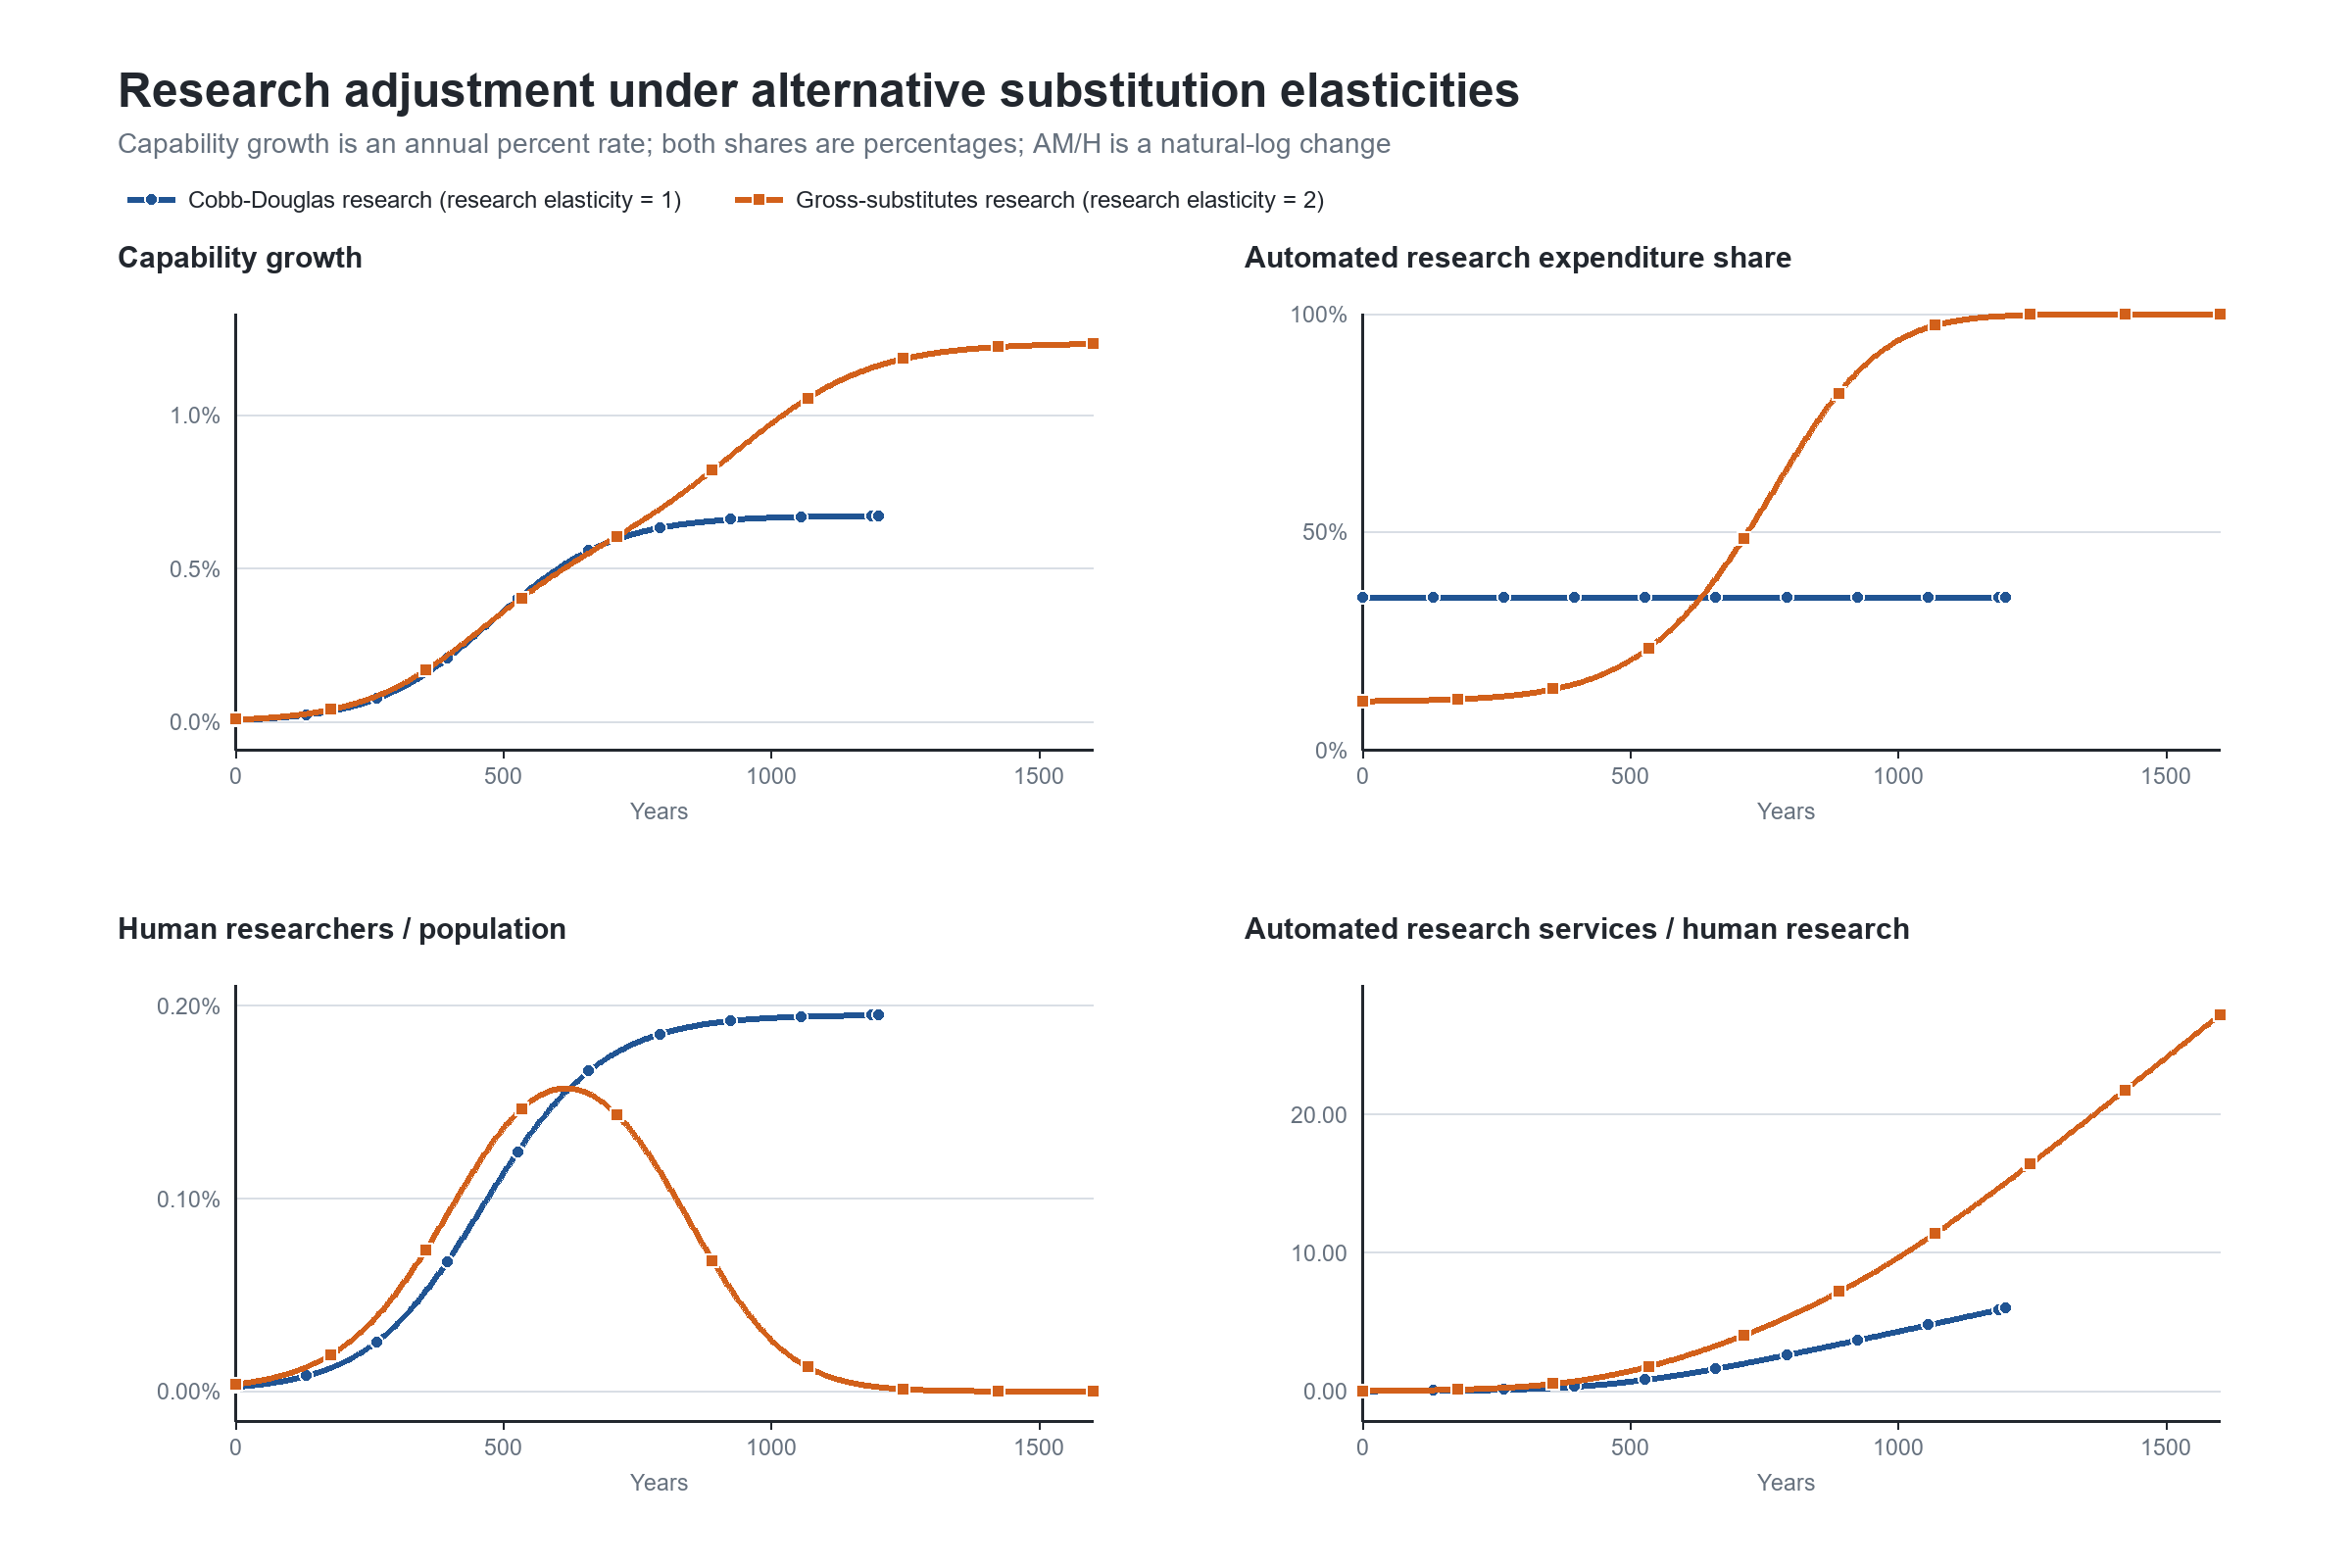
\includegraphics[width=\textwidth]{figures_axm/axm_research_technology_comparison.png}
\caption{Research substitution and the unit-elasticity balanced-growth limit.
Both lines are finite-horizon candidate-path approximations satisfying the
audited dated equilibrium conditions.
Under Proposition \ref{prop:axm-equilibrium-sufficiency}, any admissible infinite
continuation satisfying the transversality conditions would be globally optimal.}
\label{fig:axm-research-comparison}
\end{figure}

Figure \ref{fig:axm-growth-returns} focuses on the first 600 years and adds the
net real interest rate and consumption growth. The interest rate falls rapidly
toward the household discount rate and then rises as consumption-per-capita
growth rises. This comovement is required by the Euler equation,
\(r=\rho+g_{C/N}\). At the balanced-growth limit, consumption and output per
person have the same growth rate. The two research technologies produce similar returns early
in the transition and separate only as automated research becomes quantitatively
important.

\begin{figure}[H]
\centering
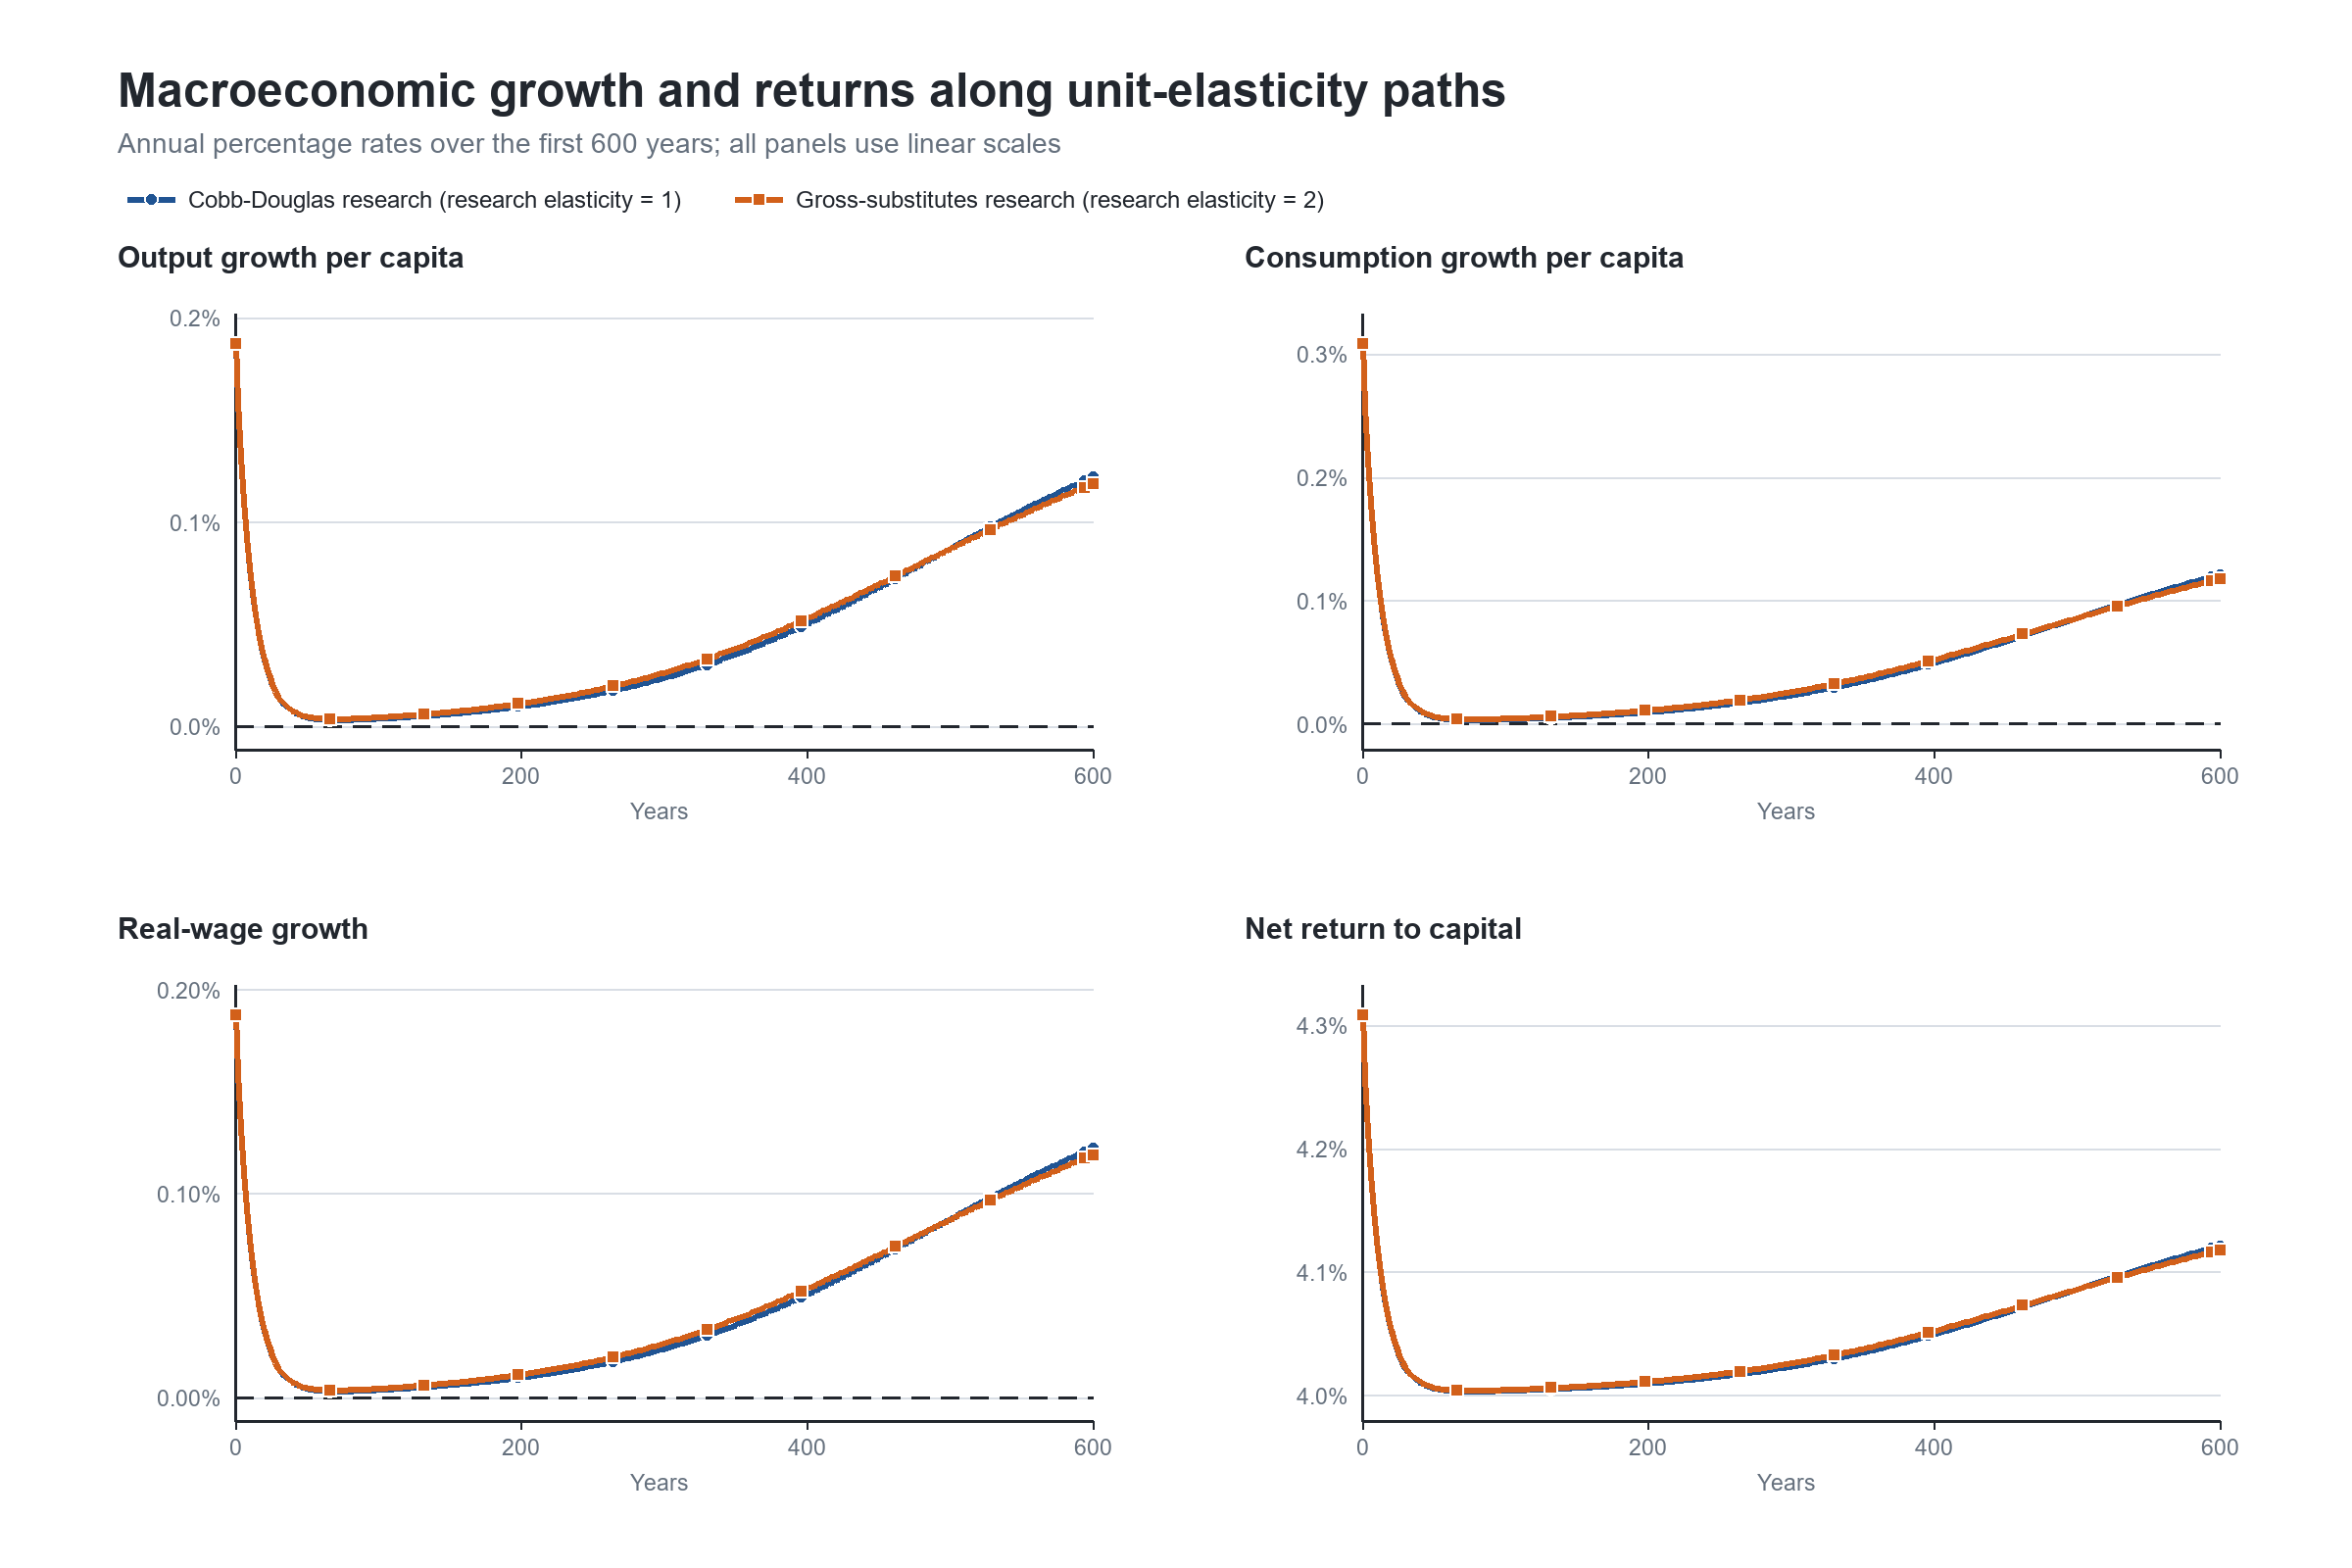
\includegraphics[width=\textwidth]{figures_axm/axm_equilibrium_growth_rates.png}
\caption{Growth rates and the net return to capital. Rates are annual percentages;
both lines are finite-horizon candidate-path approximations satisfying the
audited dated equilibrium conditions.}
\label{fig:axm-growth-returns}
\end{figure}

The path of \(H/N\) reveals a transition concealed by the limiting automated
research-expenditure share. With \(\sigma_{HM}=2\), the fraction of the population working in
AI research first rises and later falls toward zero. AI research can therefore
employ a larger share of the population during the transition even while it
becomes progressively more automated. Under Cobb--Douglas research, the human-research population share
instead converges to a positive constant.

Figure \ref{fig:axm-wages} shows that the distinction between factor prices and
factor shares already matters on these balanced-growth transitions. The real wage
eventually grows at the same rate as output per person, as Proposition
\ref{prop:axm-cd-bgp} requires. Production labor income as a share of output,
\(wL/Y\), is fixed by the Cobb--Douglas final-production technology. Aggregate
labor income as a share of output, \(wN/Y\), also includes human researchers and
therefore moves during the research-automation transition.

\begin{figure}[H]
\centering
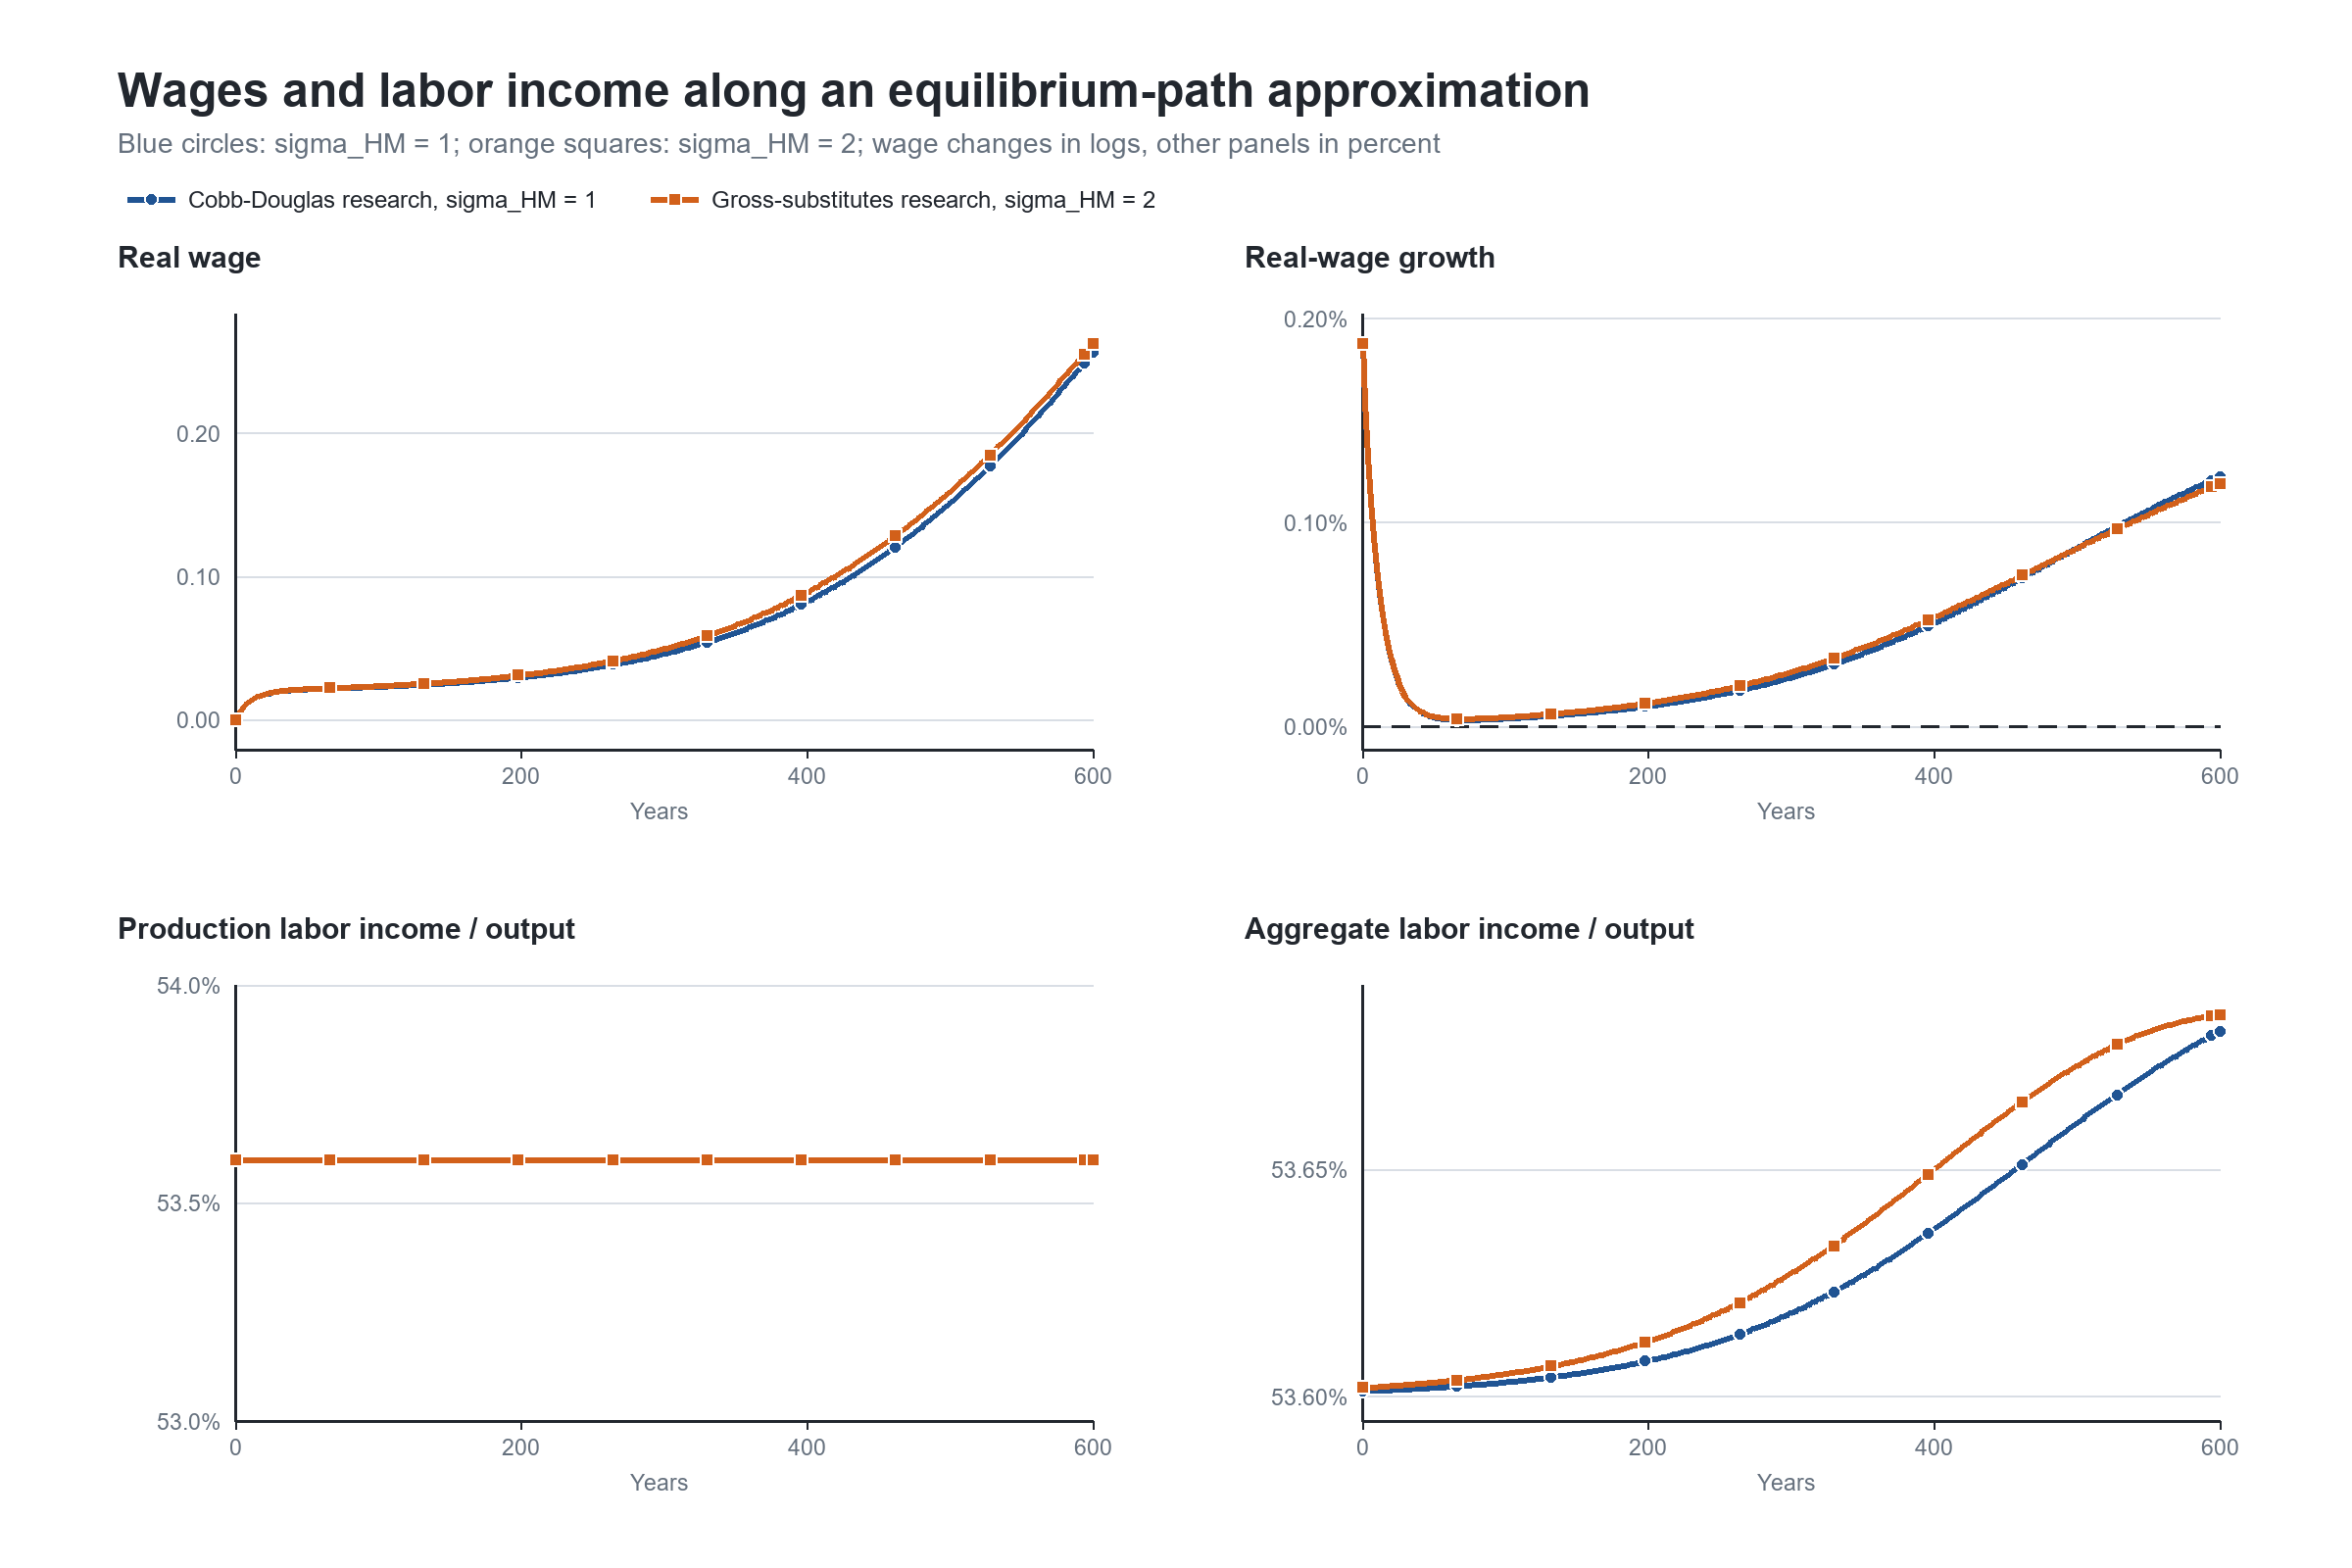
\includegraphics[width=\textwidth]{figures_axm/axm_wages_and_factor_shares.png}
\caption{Real wages and labor income along the two finite-horizon candidate-path
approximations satisfying the audited dated equilibrium conditions.}
\label{fig:axm-wages}
\end{figure}

Figure \ref{fig:axm-research-chain} separates raw research compute \(M\), the
automated services \(AM\), human research \(H\), and the effective-research
index \(E\).
This decomposition is essential for interpreting the new specification. Research
compute can grow at one rate while the services produced by that compute grow
faster because capability is improving.

\begin{figure}[H]
\centering
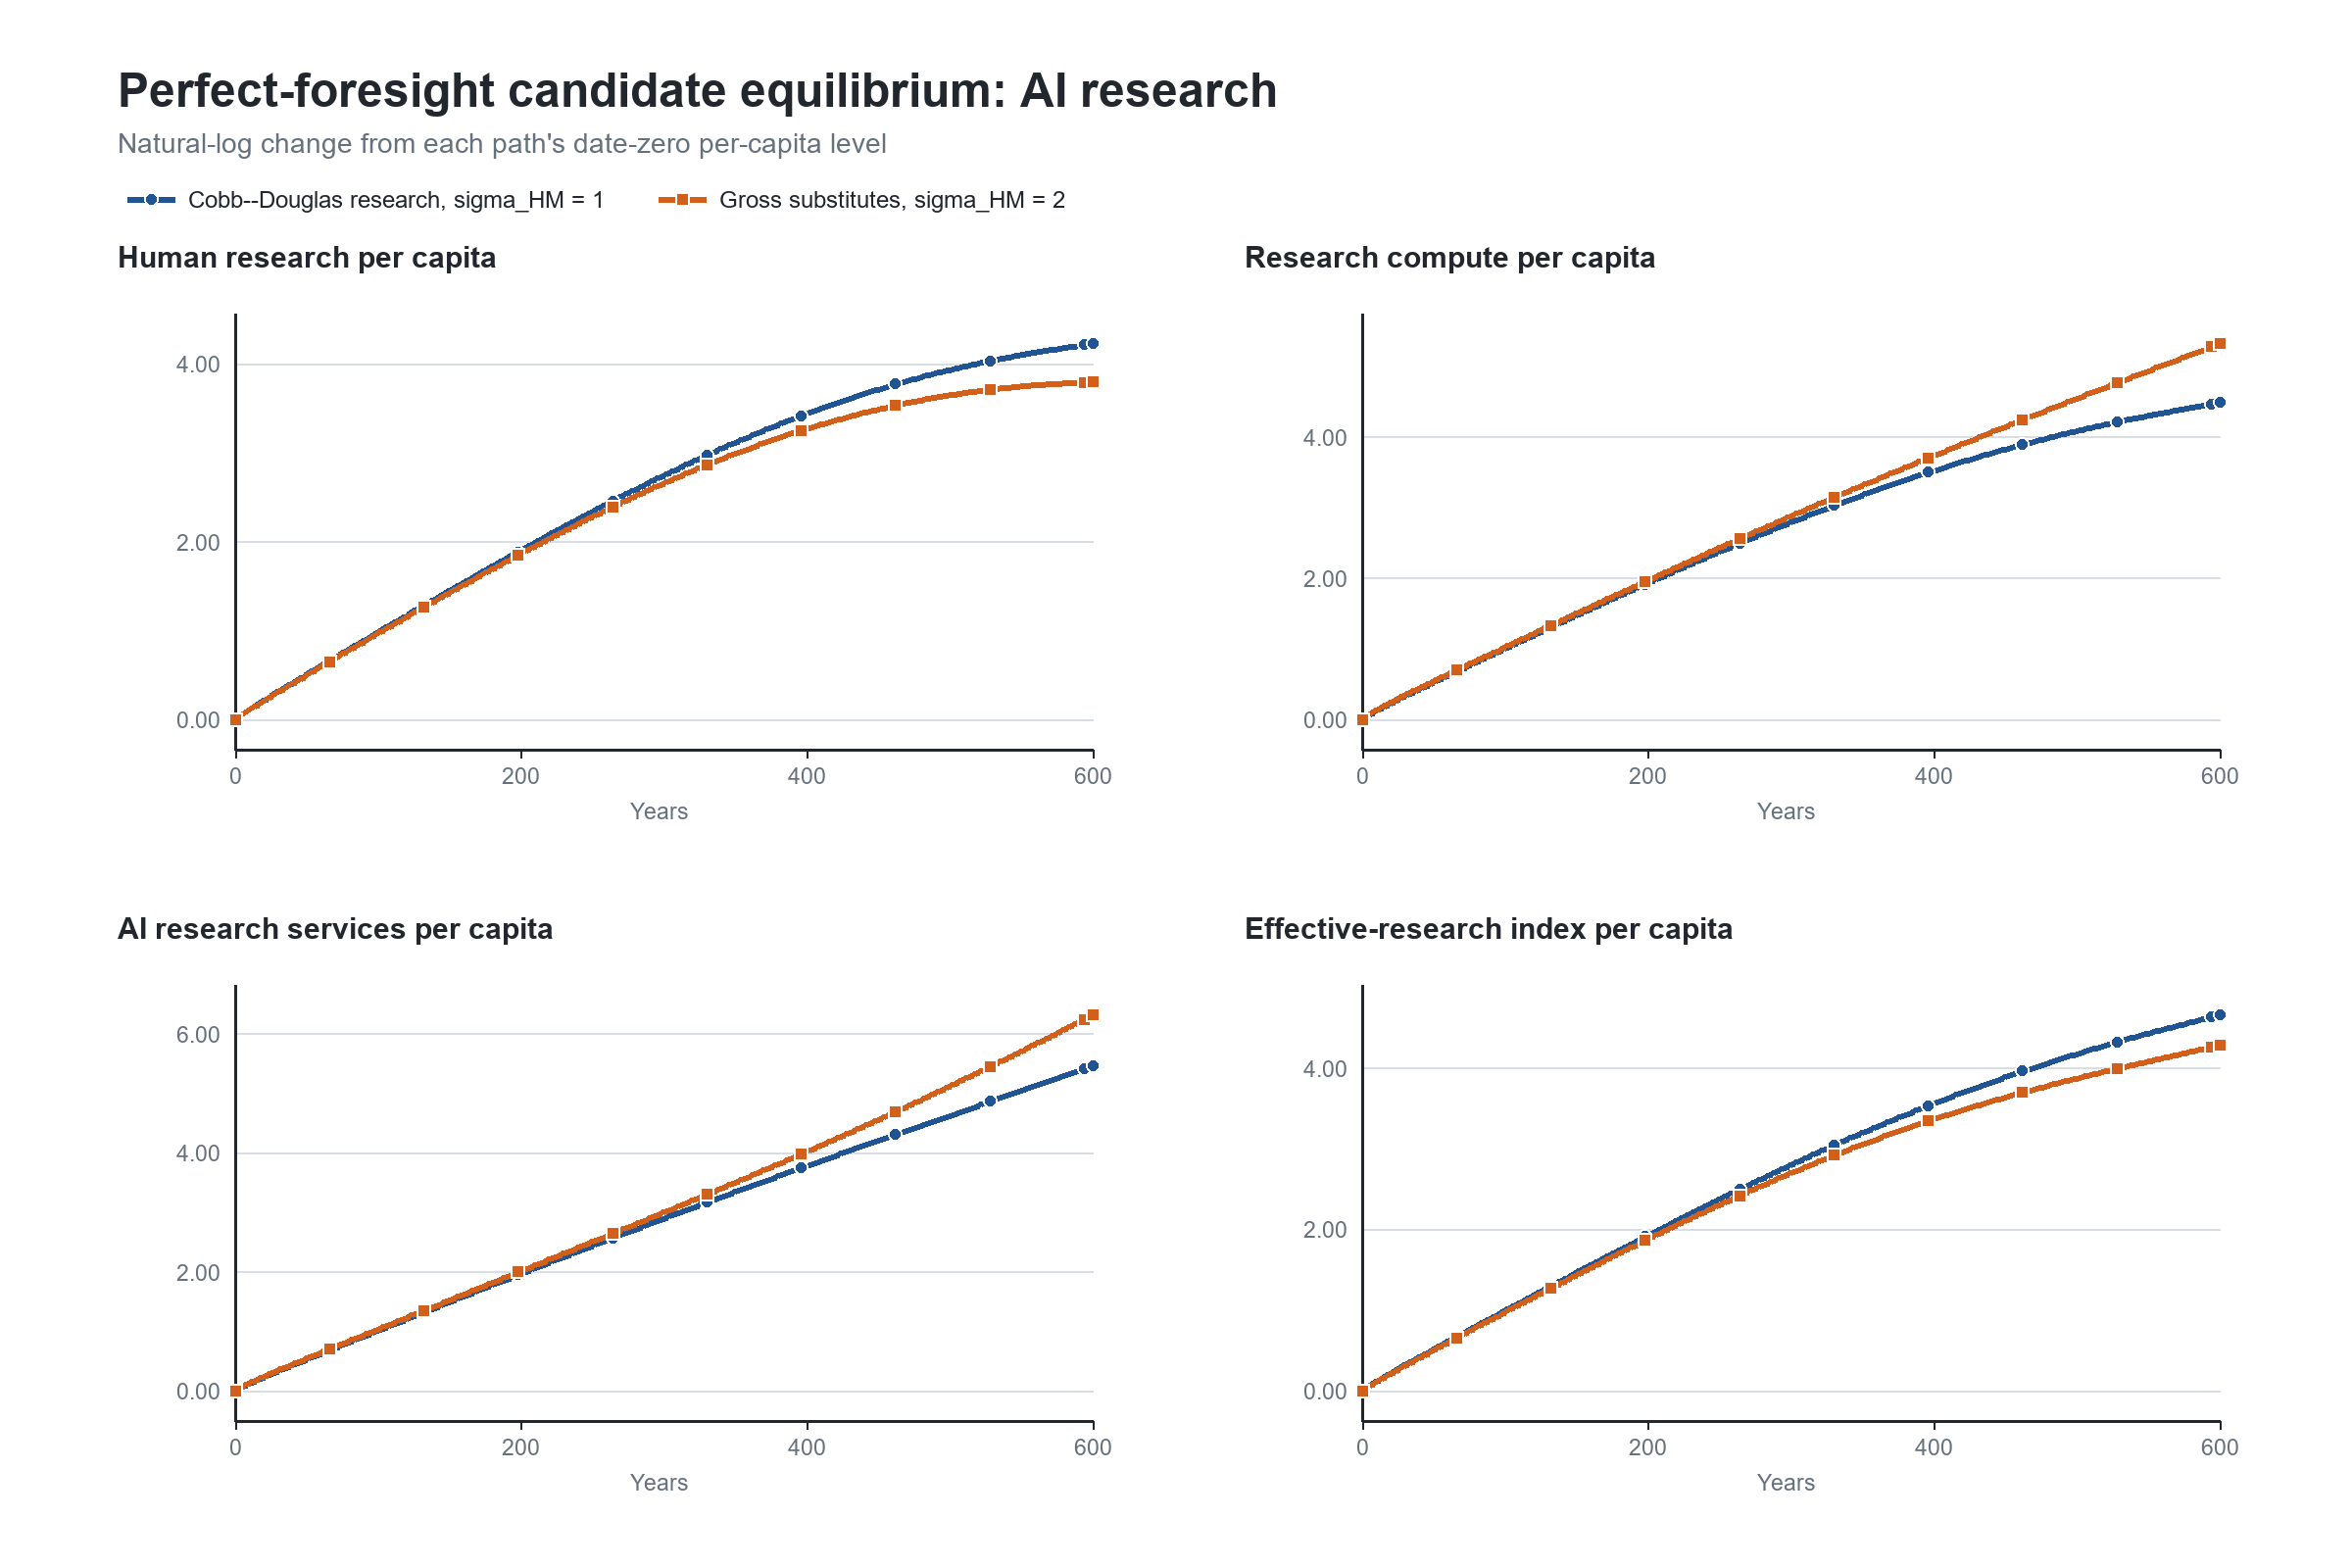
\includegraphics[width=\textwidth]{figures_axm/axm_equilibrium_research_chain.png}
\caption{The AI-research chain. The vertical axes report natural-log changes from
each path's date-zero per-capita level.}
\label{fig:axm-research-chain}
\end{figure}

\subsection{\texorpdfstring{Case IV: gross substitution in final production, \(\sigma_{XL}>1\)}{Case IV: gross substitution in final production, sigma XL > 1}}
\label{sec:axm-case-gross-substitution}

\subsubsection{Analytical characterization}

Let
\begin{equation}
 \theta=\frac{1-\alpha}{\alpha}.
 \label{eq:axm-theta}
\end{equation}
Along an interior branch with \(\sigma_{XL}>1\), \(s_X\to1\), and
\(A\to\infty\), AI services dominate the labor--AI CES aggregate. Capital
remains a separate input with elasticity \(\alpha\). The monopoly condition then
implies
\begin{equation}
 \frac{U}{Y}\to(1-\alpha)^2,\qquad
 \frac{Y}{K}\sim \mathcal D A^\theta
 \label{eq:axm-high-sigma-scaling}
\end{equation}
for a positive constant \(\mathcal D\).

\begin{proposition}[No finite-rate balanced growth with gross substitution]
\label{prop:axm-no-bgp}
Suppose \(\sigma_{XL}>1\), \(A\to\infty\), and an interior path satisfying the
necessary equilibrium conditions remains on an
interior monopoly branch on which \(s_X\to1\). Then there is no balanced-growth
path with finite constant growth rates. In particular, \(Y/K\to\infty\), so the marginal
product of capital, the net interest rate, and household consumption growth
become unbounded.
\end{proposition}

The proposition is a conditional nonexistence result. It does not prove that every
initial condition enters the assumed unbounded-capability branch: capability may
remain bounded, a globally admissible continuation may fail, or the
infinite-horizon problem may not admit an optimum. The next result characterizes
the accelerating branch when it exists.

\begin{conditionalresult}[AI-dominated singular limit]
\label{prop:axm-singular-limit}
Assume \(\sigma_{XL}>1\), \(\sigma_{HM}>1\), \(0<\eta<1\), and an
interior path satisfies all dated technology and service identities, competitive
price equations, static first- and second-order conditions, market-clearing
conditions, and canonical differential equations on its maximal time interval.
Suppose that the path approaches an AI-dominated limit, with \(A\to\infty\), \(s_X\to1\),
and \(s_M\to1\). Suppose its consumption, investment, and research-compute
shares---respectively \(C/Y\),
\((\dot K+\delta K)/Y\), and \(M/Y\)---as well as \(g_A/(Y/K)\) and \(qA/K\),
converge to positive finite limits.
Assume that the convergences of \(s_X\), \(s_M\), all the listed ratios, and the scaling ratio
\((Y/K)/(\mathcal D A^\theta)\to1\) are asymptotically regular: the growth rate
of each convergent ratio, divided by \(Y/K\), tends to zero. Write \(z=Y/K\) and
\[
 \Delta=1+\theta-\eta,\qquad
 h=\frac{\eta\alpha}{\Delta}.
\]
Then
\begin{align}
 \frac{g_A}{z}&\to h,&
 \frac{U}{Y}&\to(1-\alpha)^2,\\
 \frac{\dot K+\delta K}{Y}&\to\alpha-\theta h,&
 \frac{M}{Y}&\to\frac{\eta(1-\alpha)^2}{\Delta},\\
 \frac{qA}{K}&\to\frac{(1-\alpha)^2}{\eta\alpha},&
 \frac{C}{Y}&\to
 1-(1-\alpha)^2-\alpha+\theta h
 -\frac{\eta(1-\alpha)^2}{\Delta}.
 \label{eq:axm-singular-ratios}
\end{align}
Moreover,
\begin{equation}
 \dot z\sim\theta h z^2.
 \label{eq:axm-z-law}
\end{equation}
Because the limiting gross-investment share
\(\alpha-\theta h=\alpha(1-\eta)/(1-\alpha\eta)\) is positive, capital is
eventually increasing. Thus \(z\), and consequently output, become unbounded in
finite time.
Let
\[
 \underline\sigma=\min\{\sigma_{XL},\sigma_{HM}\}.
\]
The allocation of labor satisfies
\begin{equation}
 (H/N,L/N)\to
 \begin{cases}
  (1,0),&\sigma_{HM}<\sigma_{XL},\\
  (\bar h_N,1-\bar h_N),
      &\sigma_{HM}=\sigma_{XL}=\sigma,\\
  (0,1),&\sigma_{HM}>\sigma_{XL}.
 \end{cases}
 \label{eq:axm-singular-labor-allocation}
\end{equation}
In the equal-elasticity case, the limiting share is pinned down by
\begin{equation}
 \bar h_N=\frac{B}{1+B},\qquad
 B=\frac{\eta}{\Delta}
 \left[
  \frac{(1-\alpha)\omega_H\omega_X}{\omega_M\omega_L}
 \right]^{\sigma}.
 \label{eq:axm-singular-equal-elasticity-share}
\end{equation}
Both production labor income, \(wL/Y\), and aggregate labor income, \(wN/Y\),
vanish as shares of output, while
\begin{equation}
 \frac{g_w}{z}\to
 \frac{\alpha-(\underline\sigma-1)h}{\underline\sigma}
 \label{eq:axm-wage-limit}
\end{equation}
which is positive if and only if
\(\underline\sigma<1/(\alpha\eta)\).
\end{conditionalresult}

The result characterizes a postulated asymptotic branch of the model's necessary
conditions. Because the maximal interval ends at the singularity, it does not
establish existence or global optimality for the infinite-horizon problems, nor
does it establish that the branch is reached from arbitrary initial conditions.
Within that branch, workers move asymptotically toward the sector in which they
are harder to replace. The model delivers a sharp separation when
\(1<\underline\sigma<1/(\alpha\eta)\): aggregate labor income as a share of output
vanishes, but the wage eventually rises. Above the threshold, the same conditional
scaling implies an eventually falling wage. The case above the threshold should
not be interpreted without separately
checking monopoly optimality and convergence to the postulated branch.
At \(\underline\sigma=1/(\alpha\eta)\), the leading term in
\eqref{eq:axm-wage-limit} is zero, so this asymptotic calculation alone does not
determine the eventual direction of the wage.

\subsubsection{Audited finite-boundary candidate paths}

For the case with \(\sigma_{XL}>1\), unbounded \(A\), and \(s_X\to1\), a
conventional terminal balanced-growth condition would contradict Proposition
\ref{prop:axm-no-bgp}. We therefore use a separate
free-boundary algorithm that terminates at a large value of \(Y/K\) and imposes
two limiting ratios from Conditional Result \ref{prop:axm-singular-limit}. A path is
reported only after convergence across progressively larger terminal boundaries
and after an independent audit of the same equilibrium conditions. This prevents a
finite-horizon initial-value path from being mislabeled as an infinite-horizon
candidate equilibrium.

The reported calculation sets \(\sigma_{XL}=1.5\) and
\(\sigma_{HM}=2\), leaving every other parameter and initial stock at the values
in Table \ref{tab:axm-parameters}. The numerical objects are finite-boundary
approximations to the conditional pre-singular branch defined above: each solves
the dated necessary conditions only through its artificial terminal boundary.
Proposition \ref{prop:axm-equilibrium-sufficiency} does not cover this
parameterization. We therefore do not call the approximations an infinite-horizon
equilibrium, claim that they reach the singularity, or assert global
intertemporal optimality.

Let \(z_T\equiv(Y/K)(T)\) denote the artificial terminal boundary. The
continuation uses \(z_T=16,32,64,\) and \(128\).
Across the last doubling, both initial jump variables change by less than
\(5\times10^{-14}\). The estimated singularity date moves from 882.158 at the
first boundary to 882.175 at the last; successive changes contract from 0.0129
to 0.00316 and then 0.00077. These dates reflect the normalization of
\(\chi\), \(A_0\), and the initial stocks and are not calendar forecasts.

\begin{table}[H]
\centering
\small
\caption{Free-boundary convergence and terminal ratios,
\(\sigma_{XL}=1.5,\ \sigma_{HM}=2\)}
\label{tab:axm-high-sigma-convergence}
\begin{tabular}{lccccc}
\toprule
Terminal \(Y/K\) & 16 & 32 & 64 & 128 & Limit\\
\midrule
Estimated \(T^*\) & 882.158 & 882.171 & 882.174 & 882.175 & ---\\
\(g_A/(Y/K)\) & 0.05924 & 0.05834 & 0.05791 & 0.05771 & 0.05755\\
\(U/Y\) & 0.44393 & 0.44658 & 0.44782 & 0.44840 & 0.44890\\
\(M/Y\) & 0.08058 & 0.07936 & 0.07878 & 0.07850 & 0.07829\\
\((\dot K+\delta K)/Y\) & 0.21583 & 0.21440 & 0.21375 & 0.21344 & 0.21315\\
\(s_X\) & 0.99261 & 0.99655 & 0.99839 & 0.99925 & 1\\
\(wN/Y\) & 0.00495 & 0.00231 & 0.00108 & 0.00050 & 0\\
\bottomrule
\end{tabular}
\end{table}

Only \(C/Y\), \(qA/K\), and the terminal \(Y/K\) are imposed at each free
boundary. The remaining ratios in Table
\ref{tab:axm-high-sigma-convergence} converge toward their independently derived
analytical limits. The initial jumps and paths also converge on common calendar
intervals and on event-time windows indexed by \(Y/K\). The independent audit
reconstructs every dated equation without calling the solver's static block.
Across 11,747 saved observations, its largest static first-order-condition error
is \(1.6\times10^{-10}\), its largest saved differential-equation residual is
\(2.3\times10^{-5}\), every allocation remains strictly positive, and the
monopoly second-order margin remains positive.

Figure \ref{fig:axm-high-sigma-rates} displays the key dynamic implication. The
economy can remain close to a low-growth path for a long interval even though no
finite-rate balanced-growth limit exists on this branch. Once AI services become
quantitatively important, output-per-capita growth, capability growth,
the real-wage growth rate, and the net return to capital rise together. Consumption
per person follows the net return through the household Euler equation. The
figure stops at \(Y/K=5\) so
that the late acceleration does not compress the preceding transition.

\begin{figure}[H]
\centering
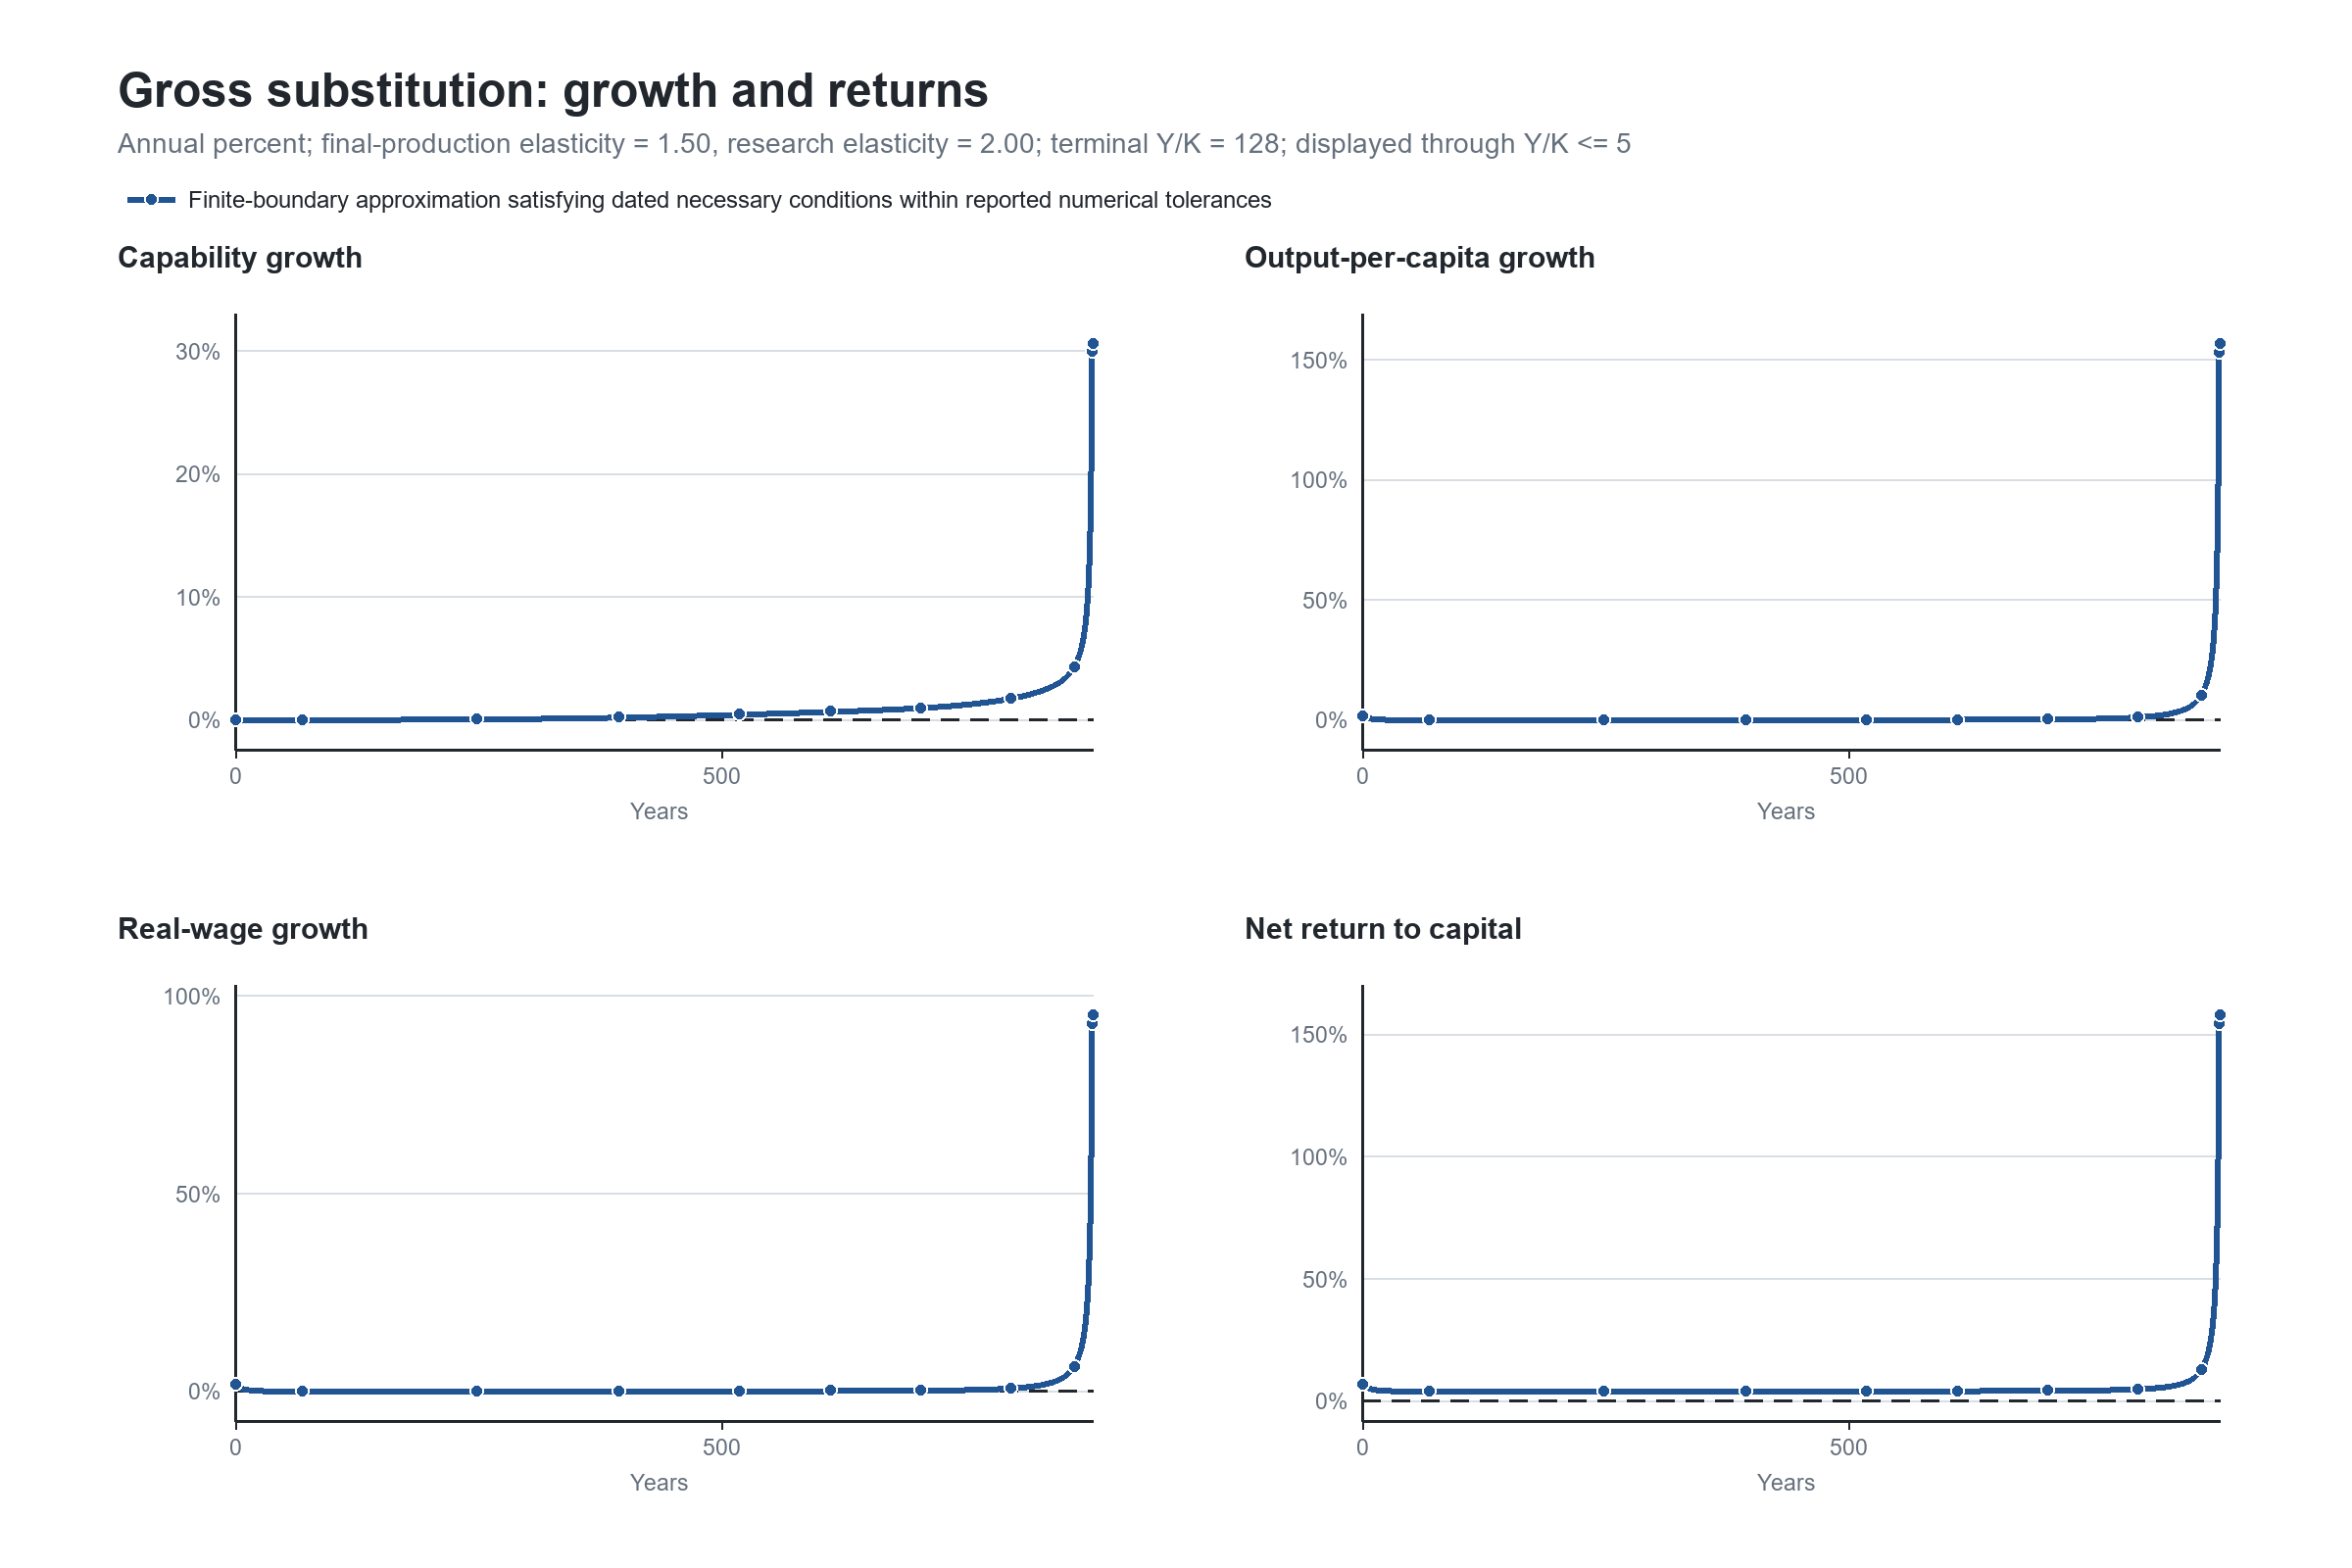
\includegraphics[width=\textwidth]{figures_axm/high_sigma_validated_transition_rates.png}
\caption{Finite-boundary approximation to the conditional pre-singular branch
for \(\sigma_{XL}=1.5\) and \(\sigma_{HM}=2\). The approximation satisfies the
audited dated necessary conditions through \(z_T=128\). Annual growth and the
net return are displayed through \(Y/K\leq5\).}
\label{fig:axm-high-sigma-rates}
\end{figure}

Figure \ref{fig:axm-high-sigma-shares} shows that automation has distinct
extensive and distributive effects. The human-research population share is
hump-shaped before tending toward zero because
\(\sigma_{HM}>\sigma_{XL}\). The automated research-expenditure share and the AI
contribution to the labor--AI composite approach one, while aggregate labor
income as a share of output approaches zero. The real wage nevertheless rises
throughout this calculation: here
\(\min\{\sigma_{XL},\sigma_{HM}\}=1.5<1/(\alpha\eta)\).

\begin{figure}[H]
\centering
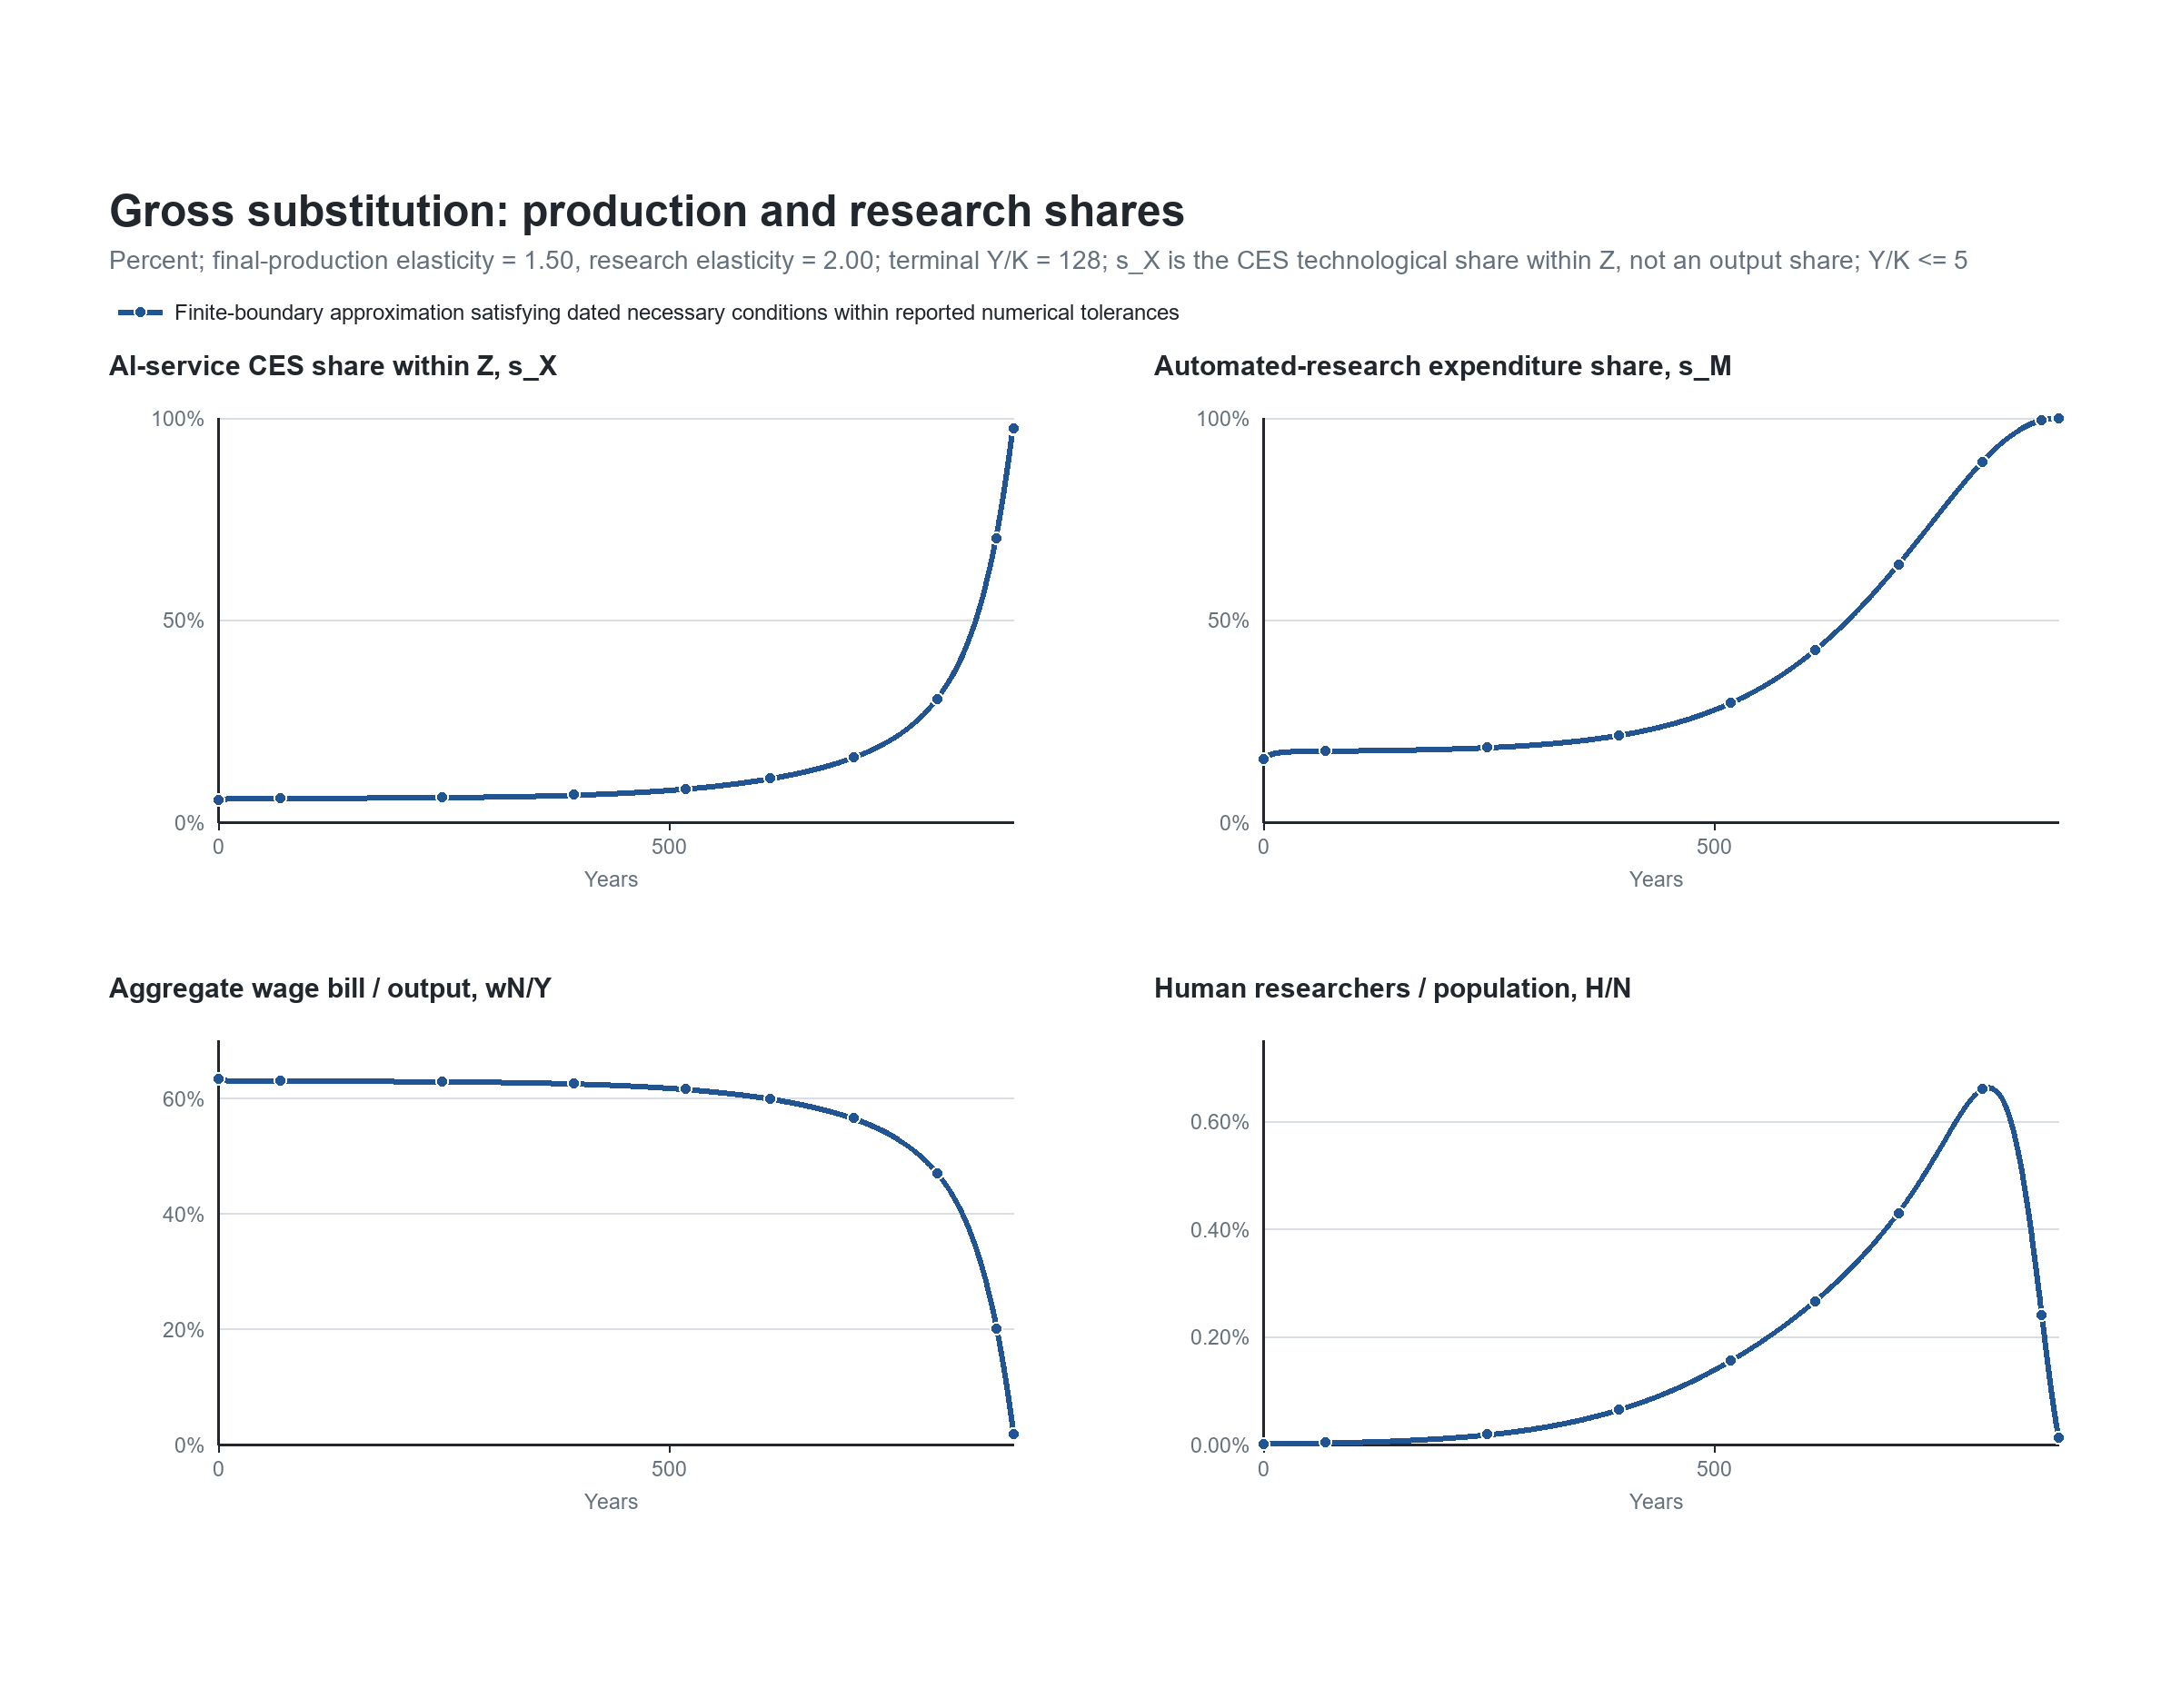
\includegraphics[width=\textwidth]{figures_axm/high_sigma_validated_transition_shares.png}
\caption{Production and research allocation along the same finite-boundary
approximation. Here \(s_X\) is AI services' elasticity within the labor--AI
composite, not their final-output income share, and \(s_M\) is the automated
research-expenditure share.}
\label{fig:axm-high-sigma-shares}
\end{figure}

The asymptotic approach is easier to see using \(Y/K\), rather than normalized
calendar time, as the event clock. Figure \ref{fig:axm-high-sigma-ratios} compares
the non-imposed ratios along the rising branch with their conditional analytical
values.

\begin{figure}[H]
\centering
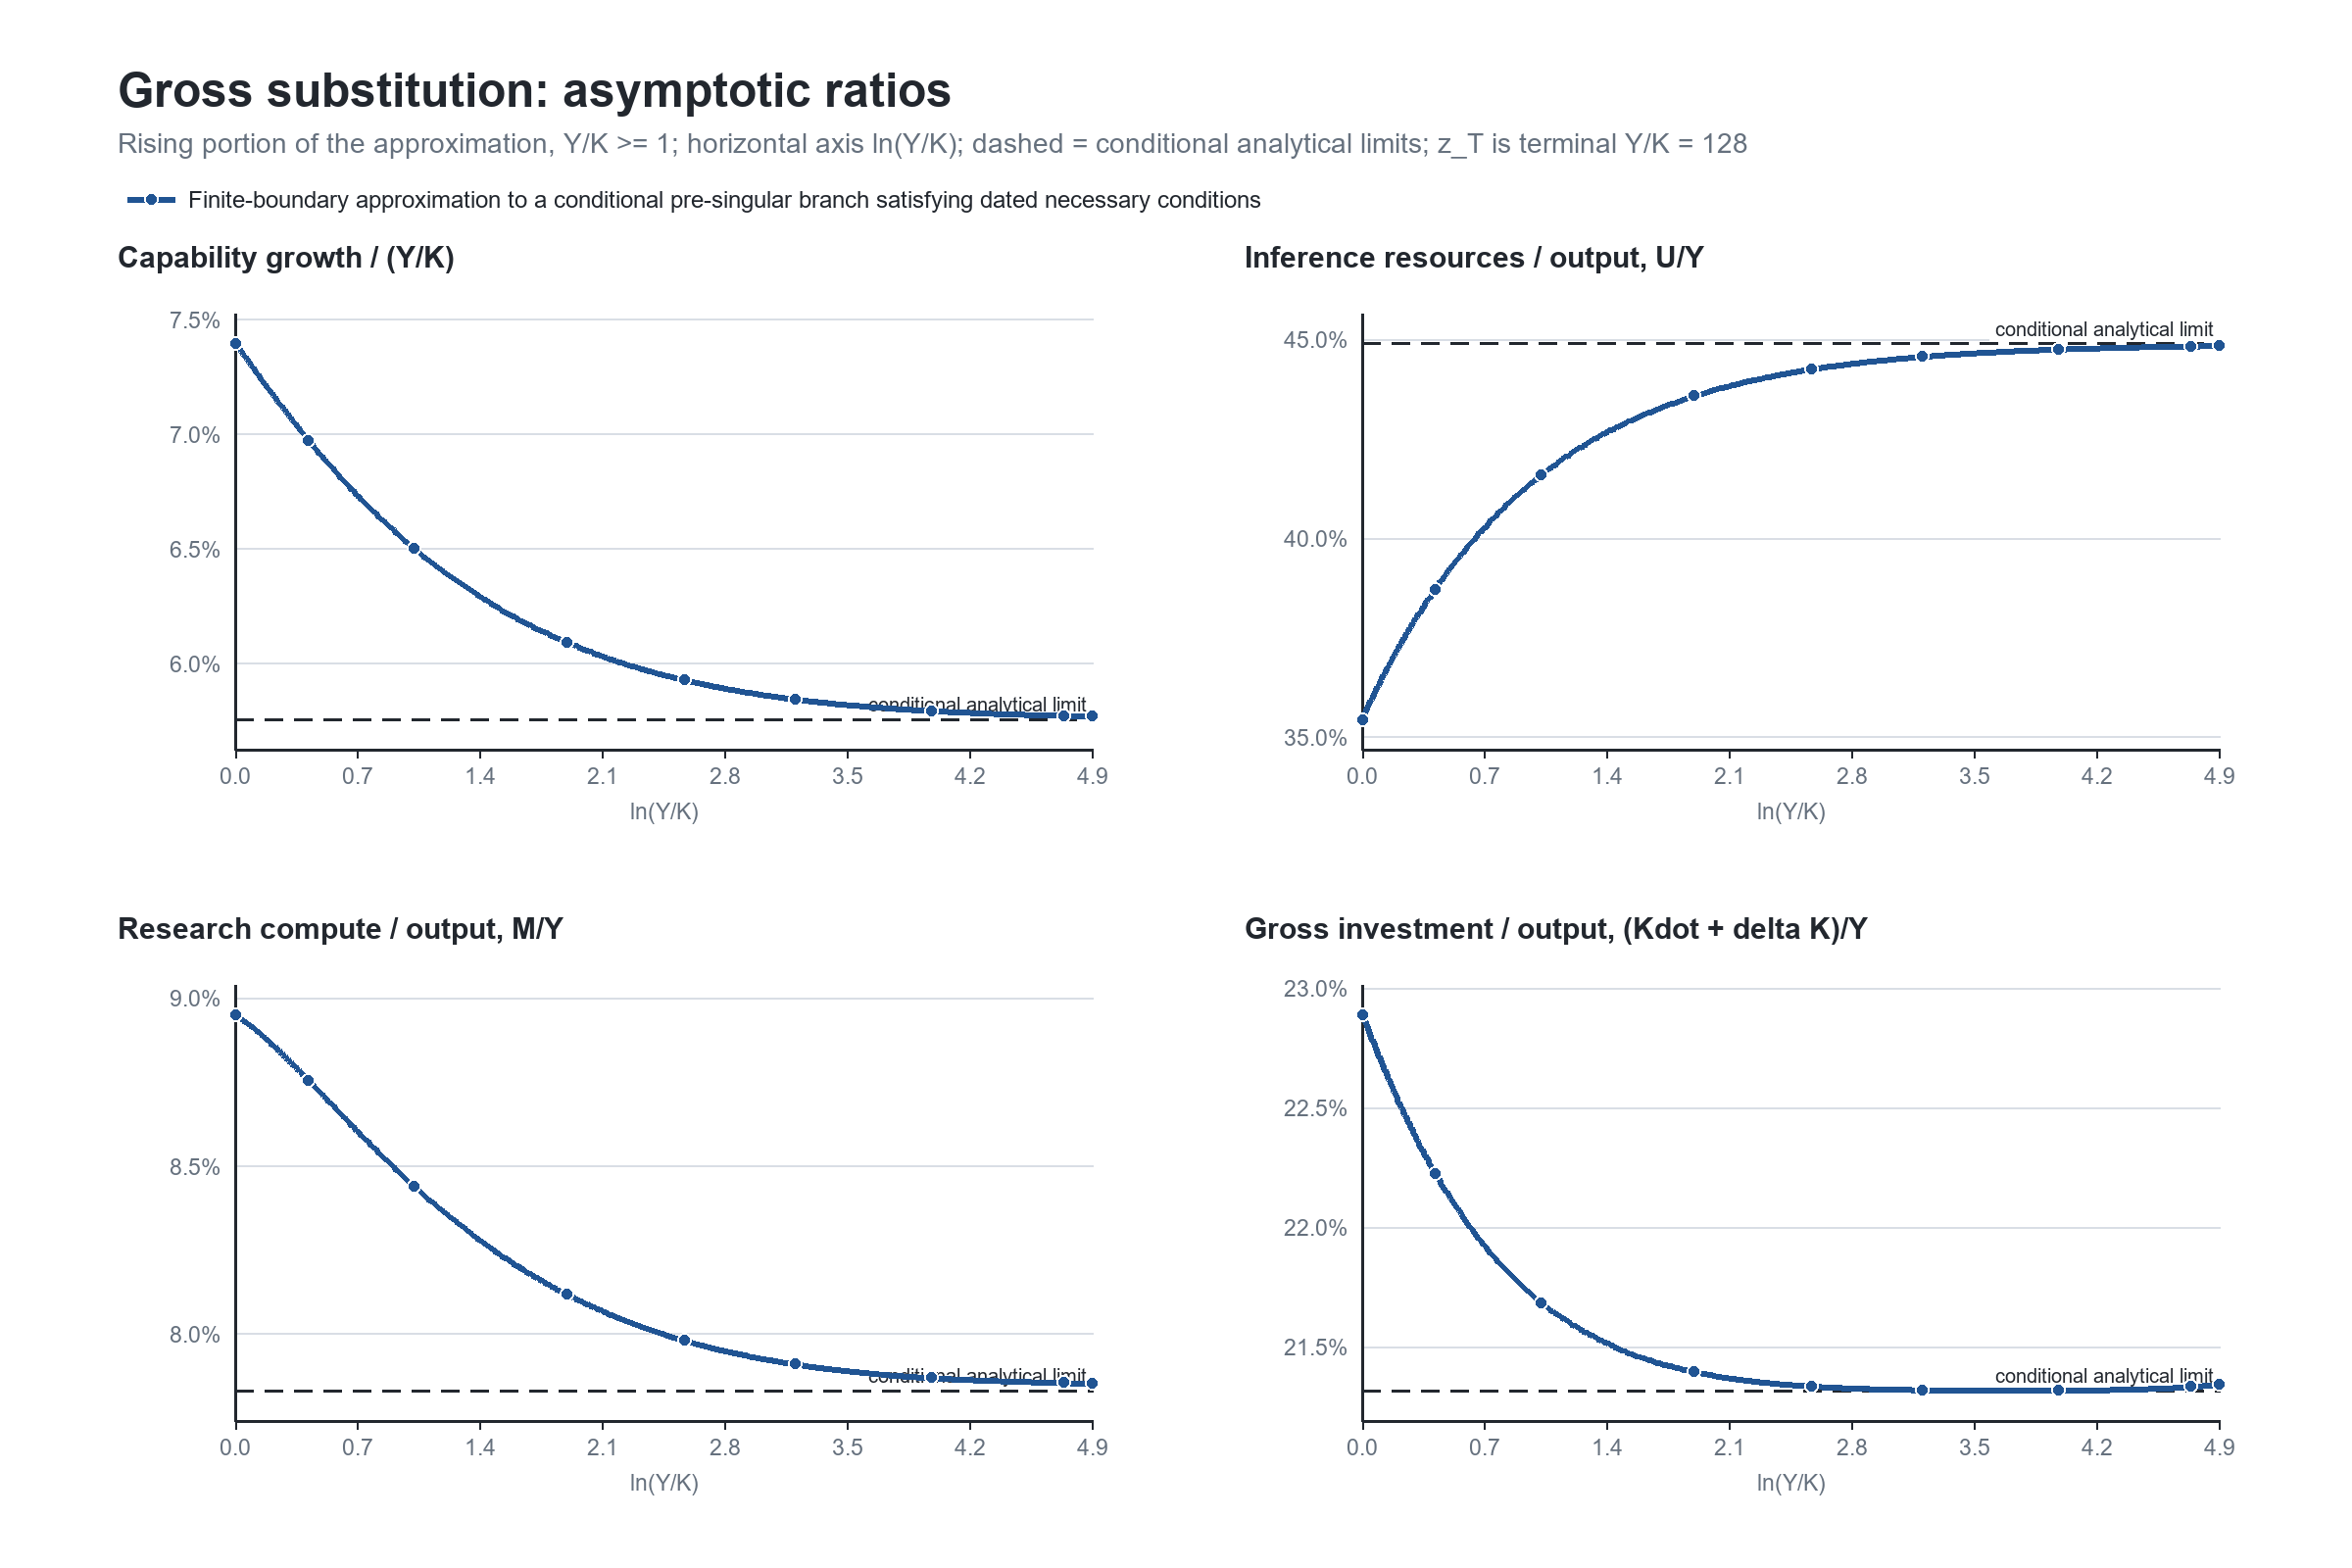
\includegraphics[width=\textwidth]{figures_axm/high_sigma_validated_asymptotic_ratios.png}
\caption{Selected ratios on the rising branch of \(Y/K\). The horizontal axis is
\(\ln(Y/K)\); dashed lines are the conditional limiting values from
Conditional Result \ref{prop:axm-singular-limit}.}
\label{fig:axm-high-sigma-ratios}
\end{figure}

\subsection{Cross-regime synthesis and limits of the evidence}

The analytical and numerical results have different evidentiary status. First,
Proposition \ref{prop:axm-research-automation} is an exact implication of the
research CES conditional demands, but its asymptotic conclusion requires the
relative-price condition \(Aw\to\infty\). Second, Proposition
\ref{prop:axm-complements} characterizes any finite-rate balanced-growth limit
satisfying its hypotheses; the paper does not provide a numerical existence or
convergence result for that regime under the present research specification.

Third, Proposition \ref{prop:axm-cd-bgp} provides necessary balanced-growth
restrictions at \(\sigma_{XL}=1\). The two audited finite-horizon paths approach
the corresponding analytical candidates and are insensitive to the reported
horizon extensions. Proposition \ref{prop:axm-equilibrium-sufficiency} establishes
global optimality for an admissible exact infinite-horizon path satisfying the
full system and transversality conditions, but the computations do not themselves
prove that such an infinite continuation exists.

Finally, Proposition \ref{prop:axm-no-bgp} rules out finite-rate balanced growth
on the stated unbounded-capability, AI-dominated branch when
\(\sigma_{XL}>1\). Conditional Result \ref{prop:axm-singular-limit} and the
free-boundary computations characterize a possible pre-singular continuation of
the dated necessary conditions. The convergence of non-imposed ratios, common
initial jumps, and common path segments supports that conditional branch; it does
not establish infinite-horizon equilibrium, global intertemporal optimality, or
selection of the branch from arbitrary initial conditions.
